\documentclass[12pt]{article}

\usepackage[no-math]{fontspec}
\usepackage{xltxtra}
\XeTeXlinebreaklocale "th_TH"
\usepackage{fonts-tlwg}
\usepackage{parskip}
\usepackage{amsmath}
\usepackage{tcolorbox}
\usepackage{listings}
\usepackage{graphicx}
\usepackage{hyperref}
\usepackage{subfig}
\usepackage{tabularx}
\usepackage{multirow}
\usepackage{xcolor, colortbl}
\usepackage{enumitem}
\usepackage{multicol}

\setmainfont[
  BoldFont={THSarabunNew_Bold.ttf},
  ItalicFont={THSarabunNew_Italic.ttf},
  BoldItalicFont={THSarabunNew_BoldItalic.ttf},
]{THSarabunNew.ttf}

\definecolor{dkgreen}{rgb}{0,0.6,0}
\definecolor{gray}{rgb}{0.5,0.5,0.5}
\definecolor{mauve}{rgb}{0.58,0,0.82}
\definecolor{codegreen}{rgb}{0,0.6,0}
\definecolor{codegray}{rgb}{0.5,0.5,0.5}
\definecolor{codepurple}{rgb}{0.58,0,0.82}
\definecolor{backcolour}{rgb}{0.95,0.95,0.92}
\definecolor{orange}{RGB}{255,127,0}

\lstset{
  frame=none,
  aboveskip=3mm,
  belowskip=3mm,
  showstringspaces=false,
  columns=flexible,
  basicstyle={\scriptsize\ttfamily},
  numbers=left, %eller none
  numberstyle=\scriptsize\color{codegray},
  keywordstyle=\color{mauve},
  commentstyle=\color{gray},
  stringstyle=\color{orange},
  breaklines=false,
  breakatwhitespace=true,
  tabsize=4,
  backgroundcolor=\color{backcolour},  
}

\hypersetup{
  colorlinks=true,
  linkcolor=blue,
  filecolor=magenta,      
  urlcolor=cyan,
  pdfpagemode=FullScreen,
}

\newcommand{\code}[1]{\texttt{\scriptsize{#1}}}
\newcommand{\bcode}[1]{\texttt{\small{#1}}}
\newcommand{\smallcode}[1]{\texttt{\tiny{#1}}}
\newcommand{\floor}[1]{\lfloor #1 \rfloor}
\newcolumntype{P}[1]{>{\centering\arraybackslash}p{#1}}

\title{รวมข้อสอบคัดผู้แทนคอมพิวเตอร์โอลิมปิกและเฉลย ปี 2020}
\author{จิรายุ บูรพาชีพ, ภาสพล เสาวคนธ์}
\date{}

\begin{document}

\maketitle

\section{Utilization}

มีเมืองอยู่จำนวน $N$ เมือง โดยแต่ละเมือง $i$ เราจะได้รับคู่อันดับจำนวน $L_i$ คู่ $(X_{i,1}, Q_{i,1}), ..., (X_{i,L_i}, Q_{i,L_i})$ จำนวน $L_i$ คู่ แทนการกระจายความน่าจะเป็นของการไฟดับ แต่ละคู่อันดับจะระบุว่า ความน่าจะเป็นที่จะมีบ้านไฟดับจำนวน $X_{i,j}$ บ้าน เท่ากับ $Q_{i,j}$  เนื่องจากเป็นการกระจายความน่าจะเป็น ผลรวมของความน่าจะเป็นสำหรับแต่ละเมืองจะมีค่าเท่ากับ $1$ เสมอ

เราต้องการจัดสรรเครื่องปั่นไฟ จำนวน $M$ เครื่อง ไปยังเมืองต่างๆ เพื่อให้ค่าคาดหวังของจำนวนเครื่องปั่นไฟที่ถูกใช้งานนั้นสูงที่สุด โดยค่าคาดหวังของการจัดสรรเครื่องปั่นไฟสามารถเขียนเป็นสมการได้ดังนี้

$$
\sum_{i=1}^{N}\sum_{j=1}^{L_i}\min(X_{i,j},assigned_i) * Q_{i,j}
$$

หาก $assigned_i$ เป็นจำนวนเครื่องปั่นไฟที่จัดสรรไปให้เมือง $i$

ข้อจำกัด: $1 \leq N \leq 100\,000, 1 \leq M \leq 300\,000$ และ $L_1 + ... + L_N \leq 300\,000$

\subsection{Subtask 1}

\underline{เงื่อนไขพิเศษ}: $L_i = 1$

เนื่องจาก $L_i=1$ เราสามารถสรุปได้ว่า $Q_{i,1}$ จะมีค่าเท่ากับ $1$ เสมอ ในกรณีนี้ สมการค่าคาดหวังจะกลายเป็น

$$
\sum_{i=1}^{N}\min(X_{i,1},assigned_i)
$$

\setlength{\fboxsep}{1em}
\fbox{\parbox{12.85cm}{
สังเกตุว่า หากปัจจุบัน $assigned_i < X_{i,1}$ แล้วเราให้เครื่องปั่นไฟเพิ่มไปอีกเครื่อง ไม่ว่าจะเพิ่มไปที่เมืองไหน ค่าคาดหวังของเราจะเพิ่มขึ้นเท่ากับ $1$ เสมอ ไม่เช่นนั้นจะเป็น $0$
}}

ดังนั้น วิธีในการให้เครื่องปั่นไฟที่ดีที่สุดคือ ให้กับเมืองใดก็ได้ที่ $assigned_i < X_{i,1}$ ไปเรื่อยๆ และคำตอบในกรณีนี้ ค่าคาดหวังจะมีค่าเท่ากับ $\min({M, \sum_{i=1}^{N}X_{i,1}})$

Total time complexity: $\mathcal{O}(N)$

\subsection{Subtask 2}

\underline{เงื่อนไขพิเศษ}: $L_i=2$ และ $X_{i,1}=0$ เสมอ

สมการค่าคาดหวังในกรณีนี้จะเท่ากับ $\sum_{i=1}^{N} \min(X_{i,2},assigned_i) * Q_{i,2}$

เราจะแก้ปัญหาเช่นเดียวกับที่ทำใน Subtask 1 โดยจะค่อยๆ เพิ่มเครื่องปั่นไฟเข้าไปเรื่อยๆ

\fbox{\parbox{12.85cm}{
สังเกตุว่าหากปัจจุบัน $assigned_i < X_{i,2}$ แล้วเราให้เครื่องปั่นไฟเพิ่มไปอีกเครื่อง ค่าคาดหวังของเราจะเพิ่มขึ้นเท่ากับ $Q_{i,2}$ ไม่เช่นนั้นจะเป็น 0
}}

ดังนั้น วิธีในการให้เครื่องปั่นไฟที่ดีที่สุดคือ ให้กับเมืองที่ $assigned_i < X_{i,2}$ และมีค่า $Q_{i,2}$ มากที่สุด ไปเรื่อยๆ เนื่องจากค่า $Q_{i,2}$ มีค่าคงที่เสมอแม้จะเพิ่มเครื่องปั่นไฟเข้าไปที่เมืองใดก็ตาม

ในส่วน Implementation นั้น เราสามารถใช้ Max-priority queue เพื่อจำลองการเลือกเมืองที่มีค่า $Q_{i, 2}$ มากที่สุดได้

Total time complexity: $\mathcal{O}(N \log N)$

\subsection{Subtask 3}

\underline{เงื่อนไขพิเศษ}: $N \leq 1\,000$ และ $M \leq 5\,000$

ในกรณีทั่วไปนั้น การเพิ่มเครื่องปั่นไฟหนึ่งเครื่องเข้าไปในเมืองที่มี $i$ ที่มี เครื่องปั่นไฟอยู่แล้วจำนวน $assigned_i$ เครื่อง

ความน่าจะเป็นที่เพิ่มขึ้นจากคู่อันดับ $(X_{i,j}, Q_{i,j})$ จะถูกแบ่งออกเป็นสองกรณีก็คือ

\begin{enumerate}
  \item $assigned_i+1 \leq X_{i,j}$ ในกรณีนี้ ค่าคาดหวังจะเพิ่มเท่ากับ $Q_{i,j}$
  \item $assigned_i+1 > X_{i,j}$ ในกรณีนี้ ค่าคาดหวังจะไม่เพิ่ม เนื่องจาก $\min$ ในสมการค่าคาดหวังบนสุด
\end{enumerate}

ดังนั้นเราสามารถสรุปได้ว่าค่าคาดหวังที่จะเพิ่มขึ้นจะมีค่าเท่ากับ $$\sum_{j \leq L_i, assigned_i+1 \leq X_{i,j}} Q_{i,j}$$

สังเกตุได้อีกว่า ยิ่ง $assigned_i$ มีค่าเยอะขึ้น ค่าคาดหวังที่จะเพิ่มขึ้นอาจจะมีค่าน้อยลงกว่าเดิม

\fbox{\parbox{12.85cm}{
วิธีในการให้เครื่องปั่นไฟที่ดีที่สุดคือ เลือกให้กับเมืองที่ มีค่า $\sum_{assigned_i+1 \leq X_{i,j}} Q_{i,j}$ มากที่สุด ไปเรื่อยๆ}}

เพราะการเลือกจัดให้กับเมืองที่มีค่าดังกล่าวที่\underline{ไม่มากที่สุด} จะไม่ทำให้คำตอบดีขึ้น เนื่องจากค่าคาดหวังที่ได้หลังจากเพิ่มเครื่องปั่นไฟให้กับเมืองนั้นไปแล้ว จะไม่เยอะขึ้น ทำให้ไม่สามารถหวังว่าจะทำให้เกิดตัวเลือกที่ดีกว่า เมืองที่มีค่าดังกล่าวมากที่สุด ในภายหลัง

ในส่วนของ Implementation ในแต่ละรอบของการเพิ่มเครื่องปั่นไฟ เราสามารถไล่ดูว่าแต่ละเมืองมีค่าดังกล่าวเท่าไหร่ แล้วเลือกจัดให้กับเมืองที่มีค่ามากที่สุด

เราสามารถคำนวณค่า $\sum_{k \leq X_{i,j}} Q_{i,j}$ สำหรับทุกค่า $i \leq N$ และ  $k \leq M$ เอาไว้ตั้งแต่แรกได้แล้ว ซึ่งสามารถคำนวณอย่างรวดเร็วได้ด้วย Suffix sum ตามตัวอย่างโค้ดภาษา \texttt{\scriptsize{C++}} ด้านล่าง

\begin{lstlisting}[language=C++]
// compute suffix sum for each town
for(int i = 1; i <= n; i++) {
  for(int j = 1; j <= L[i]; j++) sum[i][X[i][j]] += Q[i][j];
  for(int k = m-1; k >= 0; k--) sum[i][k] += sum[i][k+1];
}

// run m times
while(m--) {
  // choose the best town
  int best = 1;
  for(int i = 2; i <= n; i++) {
    if(sum[i][assigned[i]+1] > sum[best][assigned[best]+1]) best = i;
  }
  // add to the answer
  ans += sum[best][assigned[best]+1];
  assigned[best]++;
}
\end{lstlisting}

Total time complexity: $\mathcal{O}(M * N)$

\subsection{Subtask 4}

\underline{เงื่อนไข}: ไม่มีเงื่อนไขเพิ่มเติม

สังเกตุว่า ค่าของ Suffix sum ของเมือง $i$ จะเปลี่ยนค่าทุกครั้งที่ \code{k} เท่ากับ $X_{i,j}$ สำหรับบาง $j$ ดังนั้นตอนคำนวณ Suffix sum เราสามารถละทิ้งค่าในตำแหน่ง \code{k} ที่ไม่สำคัญทิ้งไปได้จำนวนมาก

ทีนี้การหาค่าของเมือง $i$ ที่จะมีเครื่องปั่นไปจำนวน $assigned_i + 1$ เครื่อง จะมีค่าเท่ากับ \texttt{\scriptsize{sum[i][up]}} โดย \texttt{\scriptsize{up}} แทน $X_{i,j}$ ที่น้อยที่สุดที่มากกว่าเท่ากับ $assigned_i + 1$ 

สุดท้าย เพื่อจำลองการเลือกเมืองที่มีค่ามากที่สุดทำได้เร็วขึ้น เราจะใช้ Max-priority queue ในการ Implement ข้อนี้

Total time complexity: $\mathcal{O}((M+N \log N)$

\newpage







































\section{Marching}

เราได้รับแผนที่ป่าซึ่งเป็นตารางขนาด $R \times C$ มา ในช่อง $(i, j)$ ใดๆ จะมีค่า $A_{i,j}$ กำกับอยู่ ซึ่งเป็นพลังงานที่ต้องใช้ในการถางป่าในช่องนั้น 

โจทย์ถามว่าเราต้องใช้พลังงานน้อยที่สุดเท่าไหร่ในการถางป่าเพื่อสร้างทางเดินที่เราสามารถเดินจากช่องมุมบนซ้าย $(1, 1)$ ไปล่างขวา $(R, C)$ และ ล่างซ้าย $(R, 1)$ ไปบนขวา $(1, C)$ ได้ โดย เส้นทางแรกจะเดินได้เพียงทิศขวาและลงล่าง ส่วน เส้นทางที่สองจะเดินได้เพียง ทิศขวาและขึ้นบน ช่องที่ถูกเดินผ่านซ้ำ จะคิดพลังงานในการถางเพียงแค่ครั้งเดียว

\begin{figure}[h]
  \centering
  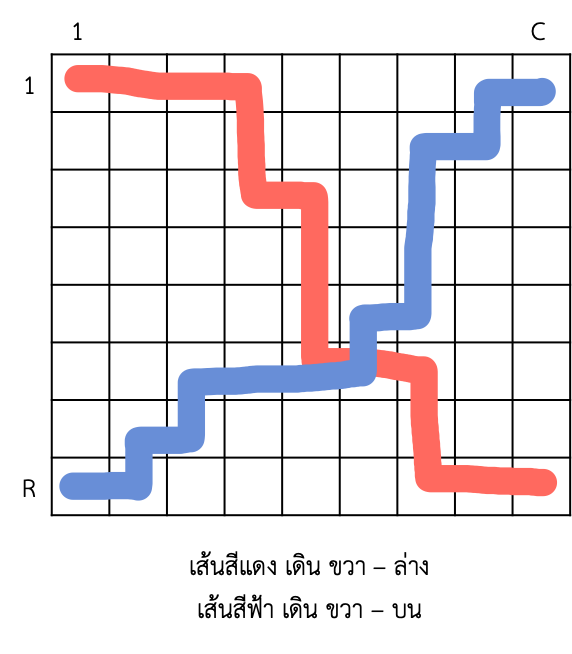
\includegraphics[height=6cm]{./images/marching1.png}
\end{figure}

\underline{ข้อจำกัด}: $R, C \leq 1\,500$

\subsection{Subtask 1}

\underline{เงื่อนไขเพิ่มเติม}: $R, C \leq 10$

\fbox{\parbox{12.85cm}{
เส้นทางเดินจาก $(1, 1)$ ไป $(R, C)$ จะตัดกับ เส้นทางจาก $(R, 1)$ ไป $(1, C)$ หนึ่งครั้งพอดี
}}

เนื่องจากโจทย์กำหนดว่าเส้นแรกจะเดินได้เพียงแค่ ขวา และ ลง และ เส้นสองเดินได้เพียงแค่ ขวา และ ขึ้น เท่านั้น ดังนั้นไม่มีทางที่เมื่อเส้นสองเส้นแยกจากกันแล้วจะวนกลับมาชนกันได้อีกครั้ง

หากเรากำหนดช่องสองช่อง $(x_1, y_1)$ และ $(x_2, y_2)$ ให้เป็นจุดเริ่มที่ทั้งสองเส้นมาชนกัน และ จุดที่แยกออกจากกัน พลังงานที่จะใช้จะมีค่าเป็น พลังงานน้อยที่สุดในการถางป่าจากมุมเริ่มต้นสองมุมมาที่ช่อง $(x_1, y_1)$ บวกกับ ช่อง $(x_2, y_2)$ ไปยังมุมจบสองมุม บวกกับ เดินจาก $(x_1, y_1)$ ไป $(x_2, y_2)$

ซึ่งระยะจากจุดใดๆไปมุม สามารถหาได้ด้วยการลองเดินจากจุดนั้นไปยังมุม ซึ่งมีจำนวน $\mathcal{O}{\binom{R+C-2}{R-1}}$ ทาง (สามารถใช้ recursive function ในการคำนวณได้)

Total time complexity: $\mathcal{O}((R*C)^2*\binom{R+C-2}{R-1})$

\subsection{Subtask 2}

\underline{เงื่อนไขเพิ่มเติม}: $R, C \leq 500$

\fbox{\parbox{12.85cm}{
เส้นทางที่ทับกันนั้นจะเป็นเส้นตรง แนวนอน หรือ แนวตั้ง เท่านั้น
}}

\begin{figure}[h]
  \centering
  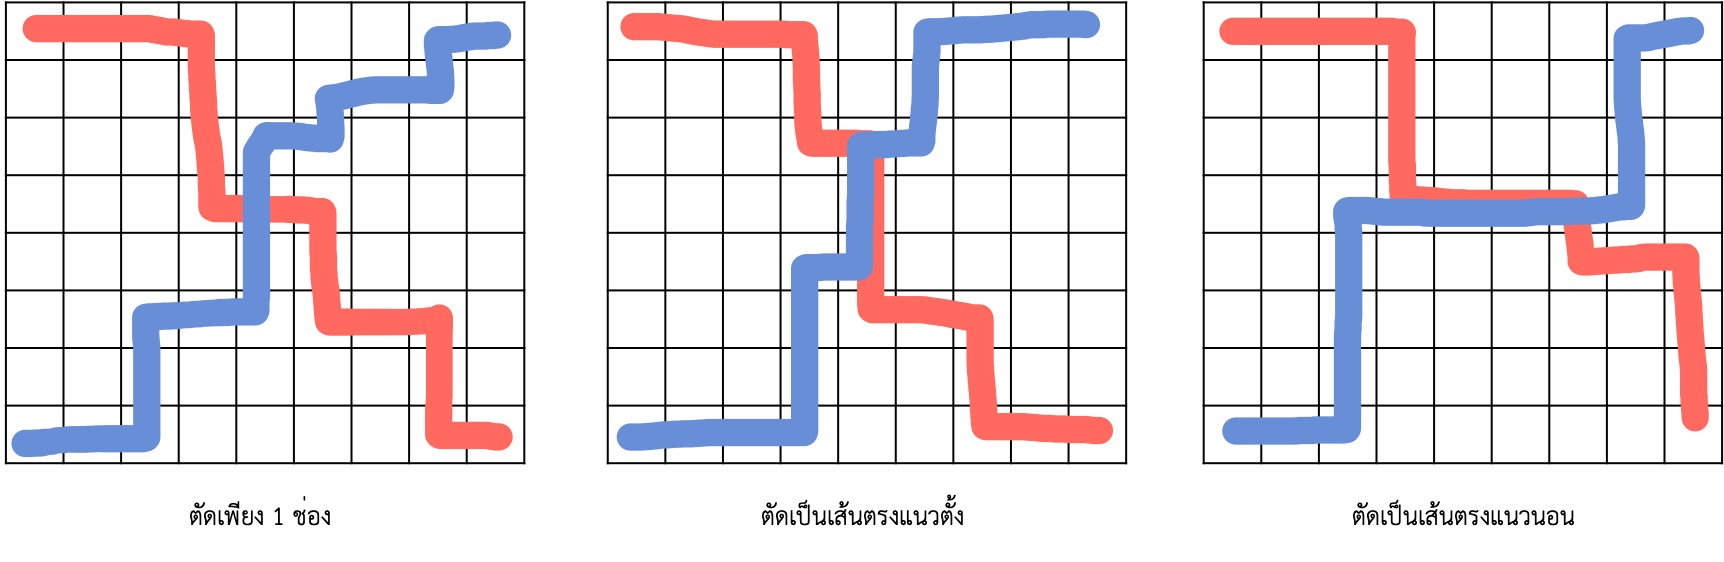
\includegraphics[height=4cm]{./images/marching2.png}
\end{figure}

เนื่องจากเส้นที่ทับกันมีลักษณะเป็นเส้นตรง การเลือกช่อง $(x_1, y_1)$ และ $(x_2, y_2)$ นี้จะมีทั้งหมด จำนวน $\mathcal{O}(R * C^2 + C * R^2)$ แบบ เนื่องจากมีสองกรณีนั่นก็คือ $x_1 = x_2$ หรือ $y_1 = y_2$

ดังนั้น เวลาที่ใช้ในการเลือกจะเหลือเพียง $\mathcal{O}(R * C^2 + C * R^2)$

นอกจากนี้ ในการคำนวณจะยะทางจากจุดมุม 4 มุมนั้น เราสามารถแก้ให้เป็น dynamic programming ได้ โดยทำการ memoize คำตอบเอาไว้ และ เราก็สามารถคำนวณพลังงานเหล่านี้ไว้ก่อนเริ่มทำการคำนวณจริงๆอีก เวลาที่ใช้ในการคำนวณพลังงานจากมุมจะเป็น $\mathcal{O}(R*C)$

\begin{lstlisting}[language=C++, title={ตัวอย่างการคำนวณพลังงานจากช่องมุมบนซ้ายไปยังทุกช่อง},captionpos=b]
for(int i = 1; i <= R; i++) {
  for(int j = 1; j <= C; j++) {
    if(i == 1 && j == 1) d1[i][j] = 0;
    else d1[i][j] = inf;
        
    if(i > 1) d1[i][j] = min(d1[i][j], d1[i-1][j] + a[i-1][j]);
    if(j > 1) d1[i][j] = min(d1[i][j], d1[i][j-1] + a[i][j-1]);
  }
}
\end{lstlisting}

Total time complexity: $\mathcal{O}(R * C^2 + C * R^2)$

\subsection{Subtask 3 และ 4}

\underline{เงื่อนไข}: ไม่มีเงื่อนไขเพิ่มเติม

กำหนดให้ \texttt{\scriptsize{d1[i][j]}}, \texttt{\scriptsize{d2[i][j]}}, \texttt{\scriptsize{d3[i][j]}} และ \texttt{\scriptsize{d4[i][j]}} แทน พลังงานที่น้อยที่สุดที่ต้องใช้ในการถางป่าจากมุมบนซ้าย, มุมบนขวา, มุมล่างซ้าย, มุมล่างขวา เพื่อมายัง ช่อง $(i,j)$ ตามลำดับ

เราจะทำการเลือกจุดเริ่มและจุดจบของเส้นที่ทับกันซึ่งคือ $(x_1, y_1)$ และ $(x_2, y_2)$ ให้เร็วขึ้น โดยในการวิเคราะห์นี้จะขอพิจารณากรณี $x_1 = x_2$ เพียงกรณีเดียว เนื่องจากวิธีการทำจะมีลักษณะคล้ายกับกรณี $y_1 = y_2$ อย่างมาก

สมมติว่า $x_1 = x_2 = x$ เราจะต้องการเลือก $y_1$ และ $y_2$ โดยที่ \texttt{\scriptsize{d1[x][y1] + d2[x][y2] + d3[x][y1] + \newline
d4[x][y2] + sum[x][y1..y2]}} มีค่าน้อยที่สุด โดย \texttt{\scriptsize{sum[x][y1..y2] = a[x][y1] + ... + a[x][y2]}}

หากเรากำหนดให้ \texttt{\scriptsize{qs[x][y] = sum[x][1..y]}} เราจะต้องการหาค่าที่น้อยที่สุดของ \texttt{\scriptsize{d1[x][y1] + d2[x][y2] + \newline d3[x][y1] + d4[x][y2] + qs[x][y2] - qs[x][y1-1]}}

ซึ่งสามารถแยกออกเป็น 2 กลุ่มได้ดังนี้ \\\
{\setlength{\fboxsep}{2pt}\fbox{$\displaystyle \texttt{\scriptsize{\newline d1[x][y1] + d3[x][y1] - qs[x][y1-1]}}$}} + {\setlength{\fboxsep}{2pt}\fbox{$\displaystyle \texttt{\scriptsize{\newline d2[x][y2] + d4[x][y2] + qs[x][y2]}}$}}

ดังนั้น ในแต่ละแถว $x$ ใดๆ หากเราไล่จากซ้ายไปขวา แล้วเก็บค่าน้อยสุดของ \texttt{\scriptsize{d1[x][y]  + d3[x][y] - qs[x][y-1]}} ใน prefix เอาไว้ แล้วเทียบกับค่า \texttt{\scriptsize{d2[x][y] + d4[x][y] + qs[x][y]}} ของตัวมันเอง เราก็จะหาค่าน้อยที่สุดของสมการยาวๆ ด้านบนได้

\begin{lstlisting}[language=C++]
int ans = inf;
for(int x = 1; x <= R; x++) {
  int best = inf;
  for(int y = 1; y <= C; y++) {
    best = min(best, d1[x][y] + d3[x][y] - qs[x][y-1]);   
    ans = min(ans, best + d2[x][y] + d4[x][y] + qs[x][y]);
  }
}
\end{lstlisting}

Total time complexity: $\mathcal{O}(R*C)$

\newpage






































\section{Pandemic}

มีประชากรจำนวน $N$ คน หมายเลข $0$ ถึง $N-1$ และ มีหนึ่งคนในนั้นเป็นผู้ติดเชื้อ 

เรามีเวลาเพียง 34 วันเพื่อที่จะหาผู้ติดเชื้อ เราได้รับสมัครอาสาสมัครจำนวน $K$ คน หมายเลข $0$ ถึง $K-1$ โดยในแต่ละวัน เราสามารถส่งอาสาสมัครไปเข้าใกล้ประชากรคนใดจำนวนกี่คนก็ได้  แต่มีข้อกำหนดว่าในแต่ละวัน ประชากรแต่ละคนจะเจออาสาสมัครได้ไม่เกิน $L$ คน

อาสาสมัครคนที่เข้าใกล้ผู้ติดเชื้อในวันที่ $i$ จะติดเชื้อและเริ่มแสดงอาการในวันที่ $i+30$ พอดี
 และห้ามไปพบประชากรอีก

ในปัญหาย่อย 4 ถึง 6 คุณจะต้องใช้อาสาสมัครให้น้อยที่สุด ถึงแม้ $K \leq 100\,000$

\underline{ข้อจำกัด}: $N \leq 100\,000$
\begin{multicols}{2}
\begin{itemize}[leftmargin=*,itemsep=1pt,parsep=1pt]
  \item ปัญหาย่อย 1: $K = 20, L = 20$
  \item ปัญหาย่อย 2: $K = 15, L = 15$
  \item ปัญหาย่อย 3: $K = 15, L = 4$
  \item ปัญหาย่อย 4: $K = 100\,000, L = 3$
  \item ปัญหาย่อย 5: $K = 100\,000, L = 2$
  \item ปัญหาย่อย 6: $K = 100\,000, L = 1$
\end{itemize}
\end{multicols}

\subsection{Subtask 1}

สำหรับคนหมายเลข $i$ หากนำเลข $i$ มาเขียนเป็นเลขฐานสองแล้ว บิท ที่ตำแหน่ง $x$ เป็น \code{1} เราจะส่งอาสาสมัครหมายเลข $x$ ไปคลุกคลีในวันที่ 1

ตัวอย่างเช่น สำหรับคนหมายเลข $101 = 1100101_2$ เราจะส่งอาสามัครคนที่ $0, 2, 5, 6$ ไปคลุกคลีในวันที่ 1

ในวันที่ 31 จะมีอาสาสมัครจำนวณหนึ่งแสดงอาการ ซึ่งหากอาสาสมัครหมายเลข $x$ แสดงอาการแสดงว่าบิทที่ $x$ ของหมายเลขผู้ติดเชื้อเป็น 1 ทำให้เราสรุปหมายเลขของผู้ติดเชื้อได้เลย

ตัวอย่างเช่น หากในวันที่ 31 เราพบว่าอาสาสมัครหมายเลข $1, 3, 6$ แสดงอาการ เราจะรู้ได้ว่าหมายเลขของผู้ติดเชื้อคือ \\\ $1001010_2 = 74$ นั่นเอง

เนื่องจากเราต้องใช้บิทจำนวน 17 บิทในการเขียน 100,000 เป็นเลขฐานสอง ดังนั้นเราจะต้องใช้อาสาสมัคร 17 คน และ แต่ละคนจะเจออาสาสมัครไม่เกิน 17 คนเช่นกัน

\subsection{Subtask 2}

เราจะแบ่งคนทั้ง $N$ คนออกเป็น 4 กลุ่มโดยแต่ละกลุ่มมีจำนวน 25,000 คน โดยคนที่ 0 ถึง 24,999 อยู่กลุ่มที่ 0 คนที่ 25,000 ถึง 49,999 อยู่กลุ่มที่ 1 เช่นนี้ไปเรื่อยๆ

เราจะส่งอาสาสมัครไปหาคนกลุ่ม 0 ในวันที่ 1, คนกลุ่ม 1 ในวันที่ 2, คนกลุ่ม 2 ในวันที่ 3 และ คนกลุ่ม 3 ในวันที่ 4  ดังนั้นจากการดูวันแรกที่มีอาสาสมัครแสดงอาการ เราสามารถบอกได้่ว่าผู้ติดเชื้ออยู่ในกลุ่มไหน

เราจะให้หมายเลขของคนที่ $i$ ในกลุ่มที่ตัวเองอยู่เป็น $i\bmod 25000 + 1$ บวก 1 เพื่อไม่ให้หมายเลขใหม่นั้นเป็น 0 ซึ่งจะทำให้มีอาสาสมัครอย่างน้อยหนึ่งคนแสดงอาการแน่นอน

ในการส่งอาสาสมัครไปหาในแต่ละวันเราจะทำเช่นเดิมกับในปัญหาย่อย 1 โดยในคราวนี้เราจะเหลือ 15 บิท ดังนั้นเราจะใช้อาสาสมัครเพียง 15 คน และ ประชากรแต่ละคนจะต้องเจออาสาสมัครไม่เกิน 15 คนเท่านั้น

ตัวอย่างเช่น

สำหรับคนหมายเลข $25111$ จะอยู่กลุ่ม 1 และ มีหมายเลขเท่ากับ $112 = 1110000_2$ เราจะส่งอาสาสมัครหมายเลข $4, 5, 6$ ไปหาในวันที่ 2 

หากมีอาสาสมัครหมายเลข $0, 2, 4$ แสดงอาการในวันที่ 33 เราจะรู้ได้ว่าผู้ติดเชื้อคือหมายเลข $10101_2 + 25000 * 2 - 1 = 50020$

\subsection{Subtask 3 ถึง 6}

ให้ $X_{i,1}, X_{i,2}, X_{i,3}, X_{i,4}$ เป็นเซ็ทของอาสาสมัครที่เจอคนที่ $i$ ในวันที่ 1, 2, 3 และ 4 ตามลำดับ เซ็ทเหล่านี้ไม่มีสมาชิกร่วมกัน เนื่องจากเราไม่ต้องการให้คนใดๆพบอาสาสมัครคนเดิมหลายครั้ง เพราะเราสนใจเพียงวันแรกที่อาสาสมัครแสดงอาการ

สมมติว่าผู้ติดเชื้อนั้นมีหมายเลข $t$ ในวันที่ 31, 32, 33 และ 34 เซ็ทของอาสาสมัครที่แสดงอาการเป็นวันแรกจะเท่ากับ \\\ $X_{t,1}, X_{t,2}, X_{t,3}$ และ $X_{t,4}$ ตามลำดับ

ดังนั้นหากเราสามารถสร้างลำดับ $X$ ขึ้นมาโดยที่ $X_i$ ของแต่ละคนไม่เหมือนของคนอื่นเลย เราจะสามารถใข้ลำดับนี้ในทั้ง การส่งอาสาสมัคร และ สรุปว่าผู้ติดเชื้อนั้นเป็นใคร ได้เลย

ให้ $M$ เป็นจำนวนอาสาสมัครที่จะใช้ในตอนสุดท้าย หาก $M = 2$ และ $L = 2$ เราจะสร้างลำดับ $X_i$ ได้ 25 แบบ

\begin{figure}[h]
  \centering
  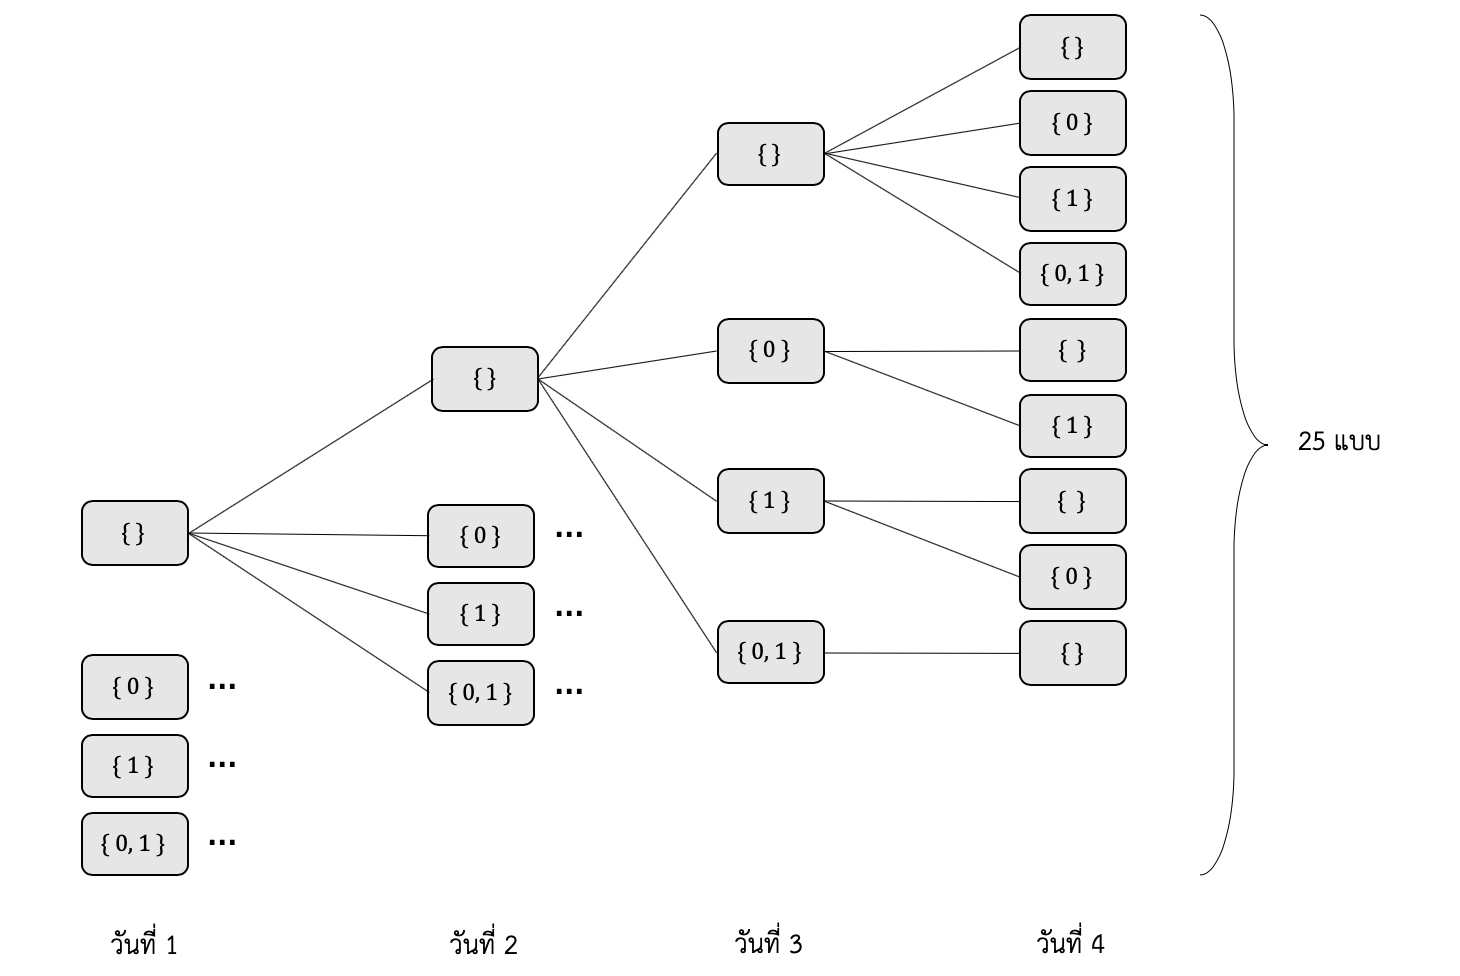
\includegraphics[height=8cm]{./images/pandemic1.png}
\end{figure}

ซึ่งทำให้ไม่สามารถใช้ $M = 2$ ได้เพราะจะมีลำดับไม่เพียงพอกับทุกคน

จากการคำนวณสามารถสรุปได้ว่า

\begin{itemize}
  \item หาก $L = 1$ ค่า $M$ ที่น้อยที่สุดที่เพียงพอคือ $19$
  \item หาก $L \geq 2$ ค่า $M$ ที่น้อยที่สุดที่เพียงพอคือ $8$
\end{itemize}

เราสามารถสร้างลำดับ $X_i$ ทั้งหมดที่เป็นไปได้นี้ออกมาด้วยการใช้ recursive function หลังจากนั้น เราสามารถทำ sequence เหล่านี้ไปใช้ในการ ถาม และ สรุปว่าผู้ติดเชื้อเป็นใครได้เลย

\begin{lstlisting}[language=C++]
// generate by calling gen(1, [0, 1, ..., m - 1])
void gen(int day, vector<int> has) {
  if(day == 5) {
    if(person < n) {
      // meet[person][i] is the set of volunteers that person meets in day i
      for(int i = 1; i <= 4; i++) {
        meet[person][i] = seq[i];
        for(auto x : seq[i]) assignments[i][x].push_back(person);
      }
      person++;
    }
    return ;
  }
  
  // choose 0
  seq[day].clear();
  gen(day + 1, has);

  // choose 1
  for(auto x : has) {
    seq[day].clear(); seq[day].push_back(x);
    vector<int> nxt;
    for(auto t : has) if(t != x) nxt.push_back(t);
    gen(day + 1, nxt);
  }
  
  // choose 2 if L >= 2
  if(lim >= 2) {
    for(auto x : has) {
      for(auto y : has) {
        if(x >= y) continue;
        seq[day].clear(); seq[day].push_back(x); seq[day].push_back(y);
        vector<int> nxt;
        for(auto t : has) if(t != x && t != y) nxt.push_back(t);
        gen(day + 1, nxt);
      }
    }
  }
}
\end{lstlisting}

\newpage

































\section{Collection}

\newpage































\section{Trainto}

รถไฟขบวนหนึ่งมีตู้โดยสาร $M$ ตู้ แต่ละตู้มีโต๊ะ 2 โต๊ะพอดี มีผู้โดยสารอีก $N$ คน โดยผู้โดยสารคนที่ $i$ จะมีึค่า $A_i$ ซึ่งแทนระดับความน่ารำคาญที่จะส่งไปให้กับทุกคนที่นั่งอยู่โต๊ะเดียวกับเขา และ นอกจากนั้นผู้โดยสารแต่ละคนจะส่งความน่ารำคาญ 1 หน่วยไปยังทุกคนที่อยู่ตู้โดยสารเดียวกับเขาด้วย 

โจทย์ต้องการให้เราจัดวางแผนที่นั่งให้ผลรวมระดับความน่ารำคาญที่ทุกคนได้รับมีค่าน้อยที่สุด

\underline{ข้อจำกัด}: $N \leq 350$ และ $2M \leq N$

\subsection{Subtask 1}

\underline{เงื่อนไขเพิ่มเติม}: $N \leq 10$

ด้วยจำนวนคนที่มีไม่เยอะ เราจึงสามารถ Brute force ทดลองวิธีในการจัดที่นั่งทั้งหมดที่เป็นไปได้ได้ ซึ่งมีจำนวน $(2M)^N$ แบบ

Total time complexity: $\mathcal{O}((2M)^N)$

\subsection{Subtask 2}

\underline{เงื่อนไขเพิ่มเติม}: $K = 1, N \leq 50$

ในปัญหาย่อยนี้ เราต้องการจัดกลุ่มคน $N$ คน ออกเป็น 2 กลุ่ม โดยที่ค่าผลรวมระดับความน่ารำคาญที่ทุกคนได้รับมีค่าน้อยที่สุด

นั่นคือ หากให้ $CNT_i$ และ $SUM_i$ แทนจำนวนคน และ ผลรวมระดับความน่ารำคาญ ของคนกลุ่ม $i$ ตามลำดับ เราต้องการที่จะทำให้ค่า $CNT_1 * SUM_1 + CNT_2 * SUM_2 + 2 * CNT_1 * CNT_2$ น้อยที่สุด

สมมติว่าเรารู้ค่า $CNT_1$ และ $CNT_2$ ในการจัดกลุ่มที่ดีที่สุดแล้ว เราจะหาวิธีการจัดคนเข้าไปในแต่ละกลุ่มที่ดีที่สุด

\fbox{\parbox{12.85cm}{
หาก $A_x > A_y$ แล้ว $x$ จะอยู่ในกลุ่มที่\underline{ไม่ใหญ่ไปกว่า}กลุ่มของ $y$ เสมอ
}}

เนื่องจาก หาก $x$ อยู่ในกลุ่มที่ใหญ่กว่า $y$ เราสามารถสลับ $x$ กับ $y$ เพื่อให้ค่าความน่ารำคาญน้อยลงได้

ดังนั้น เราเพียงแค่เรียงคนจากมากไปน้อย แล้วลองกำหนดค่า $CNT_1$ ทุกกรณี ($CNT_2 = N-CNT_1$ และ $CNT_1 \leq CNT_2$) ก็จะสามารถคำนวณผลรวมระดับความน่ารำคาญได้

Total time complexity: $\mathcal{O}(N \log N)$

\subsection{Subtask 3}

\underline{เงื่อนไขเพิ่มเติม}: $A_i$ เท่ากันหมด, $N \leq 50$

เนื่องจากทุกคนมีความน่ารำคาญเท่ากัน ดังนั้นเราจะสนใจเพียงแค่ขนาดของแต่ละโต๊ะในแต่ละตู้โดยสารเท่านั้น

เราสามารถนำผู้โดยสารทั้งหมดมาเรียงเป็นเส้นตรง แล้วแบ่งเป็น $2K$ ช่วง โดยช่วงที่ 1 และ 2 อยู่ตู้โดยสารแรก ช่วงที่ 3 และ 4 อยู่ตู้โดยสารที่สอง ไปเรื่อยๆ

เราสามารถใช้ Dynamic programming ในการแก้ปัญหาได้โดยกำหนดให้ \code{dp[x][k]} แทนผลรวมค่าความน่ารำคาญที่น้อยที่สุดสำหรับการแบ่ง \code{x} คนแรก ไปใน \code{k} ตู้โดยสาย ซึ่งสามารถเขียนเป็นสมการได้ดังนี้

\begin{center}
\code{dp[0][0] = 0} และ \code{dp[0][i] = inf} สำหรับ \code{i} ใดๆที่ไม่ใช่ 0

\code{dp[x][k] = min(dp[y-1][k-1] + cost(y,x)))} โดย 1 ≤ \code{y} ≤ \code{x}
\end{center}

\code{cost(l,r)} คือค่าความน่ารำคาญน้อยที่สุดสำหรับการแบ่งคนตั้งแต่ $l$ ถึง $r$ ออกเป็นสองส่วน ซึ่งทำเหมือนกับใน Subtask 2

Total time complexity: $\mathcal{O}(N^3 + N^2*K)$

\subsection{Subtask 4}

\underline{เงื่อนไขเพิ่มเติม}: $N \leq 50$

สมมติว่าเราได้แบ่งคนออกเป็น $2K$ กลุ่มแล้ว เราจะต้องจับคู่กลุ่ม $2K$ กลุ่มนี้ออกเป็น $K$ คู่ เพื่อจัดไปในแต่ละตู้โดยสาร

\fbox{\parbox{12.85cm}{
การจับคู่ที่ดีที่สุดคือการจับคู่กลุ่มที่เล็กที่สุด กับ กลุ่มที่ใหญ่ที่สุด กลุ่มที่เล็กสุดถัดมา กับ กลุ่มเล็กสุดกลุ่มถัดมา ไปเรื่อยๆ จนหมด
}}

\begin{figure}[h]
  \centering
  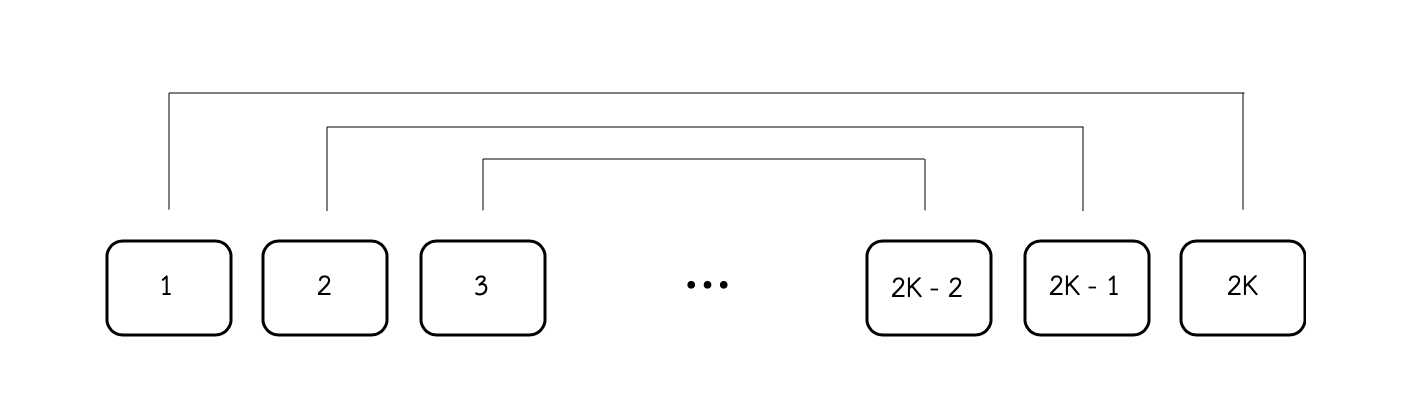
\includegraphics[height=3cm]{./images/trainto.png}
\end{figure}

เช่นเดียวกับใน Subtask 2 ถ้าหากเรานำผู้โดยสารทั้งหมดมาเรียงเป็นเส้นตรงจากระดับความน่ารำคาญมากไปน้อย แล้วแบ่งกลุ่มเป็น $2K$ ขนาดของกลุ่มจะใหญ่ขึ้นไล่ไปเรื่อยๆจากกลุ่มแรกจนถึงกลุ่มสุดท้าย

ดังนั้น เราสามารถจับคู่กลุ่มแรก กับ กลุ่มสุดท้าย และ กลุ่มสอง กับ กลุ่มรองสุดท้าย ไปเรื่อยๆ ได้เลย

เราสามารถใช้ Dynamic programming เพื่อแก้ปัญหาย่อยนี้เพียงแค่รู้ว่ากลุ่มหน้ากลับกลุ่มหลังจับคู่กันจะได้คำตอบที่ดีที่สุดได้ โดย \code{dp[k][l][r]} คือความน่ารำคาญน้อยที่สุดหากแบ่งคนตั้งแต่ $l$ ถึง $r$ ออกเป็น $k$ กลุ่ม

\begin{center}
\code{dp[k][l][r] = min(dp[k-1][x+1][y-1] + \\\ (x-l+1)*sum[l..x] + (r-y+1)*sum[y..r]) + 2*(x-l+1)*(r-y+1))} \\\
โดย \code{l} ≤ \code{x} < \code{y} ≤ \code{r}
\end{center}

Total time complexity: $\mathcal{O}(N^4*K)$


\subsection{Subtask 5 และ 6}

\underline{เงื่อนไข}: ไม่มีเงื่อนไขเพิ่มเติม

จาก Subtask 5 เรารู้ว่า ขนาดของช่วงน้อยจะมีขนาดน้อยไปมาก หากเรียงคนด้วยค่ามากไปน้อย

\fbox{\parbox{12.85cm}{
ช่วงที่ $K$ จะมีขนาดไม่เกิน $N/K$ เสมอ
}}

เนื่องจากขนาดของช่วงที่ $K+1, ..., 2K$ จะมีขนาดอย่างน้อยเท่ากับขนาดของช่วงที่ $K$ หากขนาดของช่วงที่ $K$ มีขนาด $N/K + 1$ ผลรวมขนาดของช่วงหลังจะมีค่าอย่างต่ำ $N + K$ ซึ่งเกินจำนวนคนทั้งหมดที่มี และ เป็นไปไม่ได้

ดังนั้น ใน Loop ของ \code{x} ซึ่งแทนจำนวนคนในกลุ่มหน้าจะวนไม่เกิน $\mathcal{O}(N/k)$ ก็พอ ทำให้เราตัด $K$ ออกไปจาก Time complexity ได้

Total time complexity: $\mathcal{O}(N^4)$

\subsection{Challenge}

เราอาจะเพิ่มความเร็วของอัลกอริธึมได้ด้วย Divide and conquer optimization เป็น $\mathcal{O}(N^3 \log N)$

\newpage


































\section{Racing}

มีรถแข่ง $N$ คัน หมายเลข $1$ ถึง $N$  กำลังออกตัวจากจุดเริ่มต้นของสนามแข่งรถที่มีความยาวไม่จำกัด $N$ เลน ซึ่งความเร็วเริ่มต้นของรถคันที่ $i$ เท่ากับ $U_i$ เมตรต่อวินาที โดยที่ $U_i$ เป็นจำนวนเต็มที่ $1 \leq U_i \leq 5$

นอกจากนั้น มีเหตุการณ์เกิดขึ้น $M$ เหตุการณ์ ซึ่งเป็นไปได้สองแบบดังนี้

\begin{enumerate}
  \item ที่เวลา $T$ มีการขุดหลุมในเลน $A$ ถึง $B$ ที่ระยะ $X$ จากจุดเริ่มต้น $(1 \leq T < 10^8, 1 \leq X \leq 10^9)$\\\
  รถที่มาถึงหลุมพอดีในเวลานั้นหรือช้ากว่าจะตกหลุมทำให้ขยับไปไหนไม่ได้อีก 
  \item ที่เวลา $T$ ทำการปรับความเร็วรถในเลน $A$ ถึง $B$ ให้มีความเร็วไม่เกิน $V$ $(1 \leq T < 10^8, 1 \leq V \leq 5)$ \\\
  รถคันใดที่มีความเร็วไม่เกิน $V$ อยู่แล้วจะไม่มีผลกระทบใดๆ และ $V$ เป็นจำนวนเต็ม
\end{enumerate}

เราอยากทราบว่าเมื่อเวลาผ่านไป $10^8$ วินาที รถแต่ละคันจะอยู่ที่ตำแหน่งใด

\underline{ข้อจำกัด}: $1 \leq N \leq 100\,000$ และ $0 \leq M \leq 200\,000$

\subsection{Subtask 1}

\underline{เงื่อนไขเพิ่มเติม}: $N \leq 1\,000$ และ $M \leq 1\,000$

สำหรับรถหมายเลข $x$ ใดๆ เราต้องการหา $T_{x,1}, T_{x,2}, ..., T_{x,5}$ ซึ่งเป็นเวลาที่รถคันนี้เปลี่ยนความเร็วเป็นไม่เกิน $1, 2, ..., 5$ ดามลำดับ 
$$
T_{x,i} = 
\begin{cases}
  1 
  & i \geq U_x\\
  \min(T_y) 
  & \text{สำหรับการปรับความเร็ว } y \text{ ที่ } A_y \leq x \leq B_y \text{ และ } i \geq V_y \\
  10^8 + 1
  & i = 0
\end{cases}
$$
รถคันที่ $x$ จะตกหลุมที่ตำแหน่ง $\min(X_y)$ สำหรับทุกหลุม $y$ ที่ $A_y \leq x \leq B_y$ และ มีบาง $i$ ที่\\\
$S_{x,i} + (T_y - T_{x,i}) * i \leq X_y$ เนื่องจาก ฝั่งซ้ายเป็นระยะทางที่เดินทางได้ใน $T_y$ วินาที และ น้อยกว่าเท่ากับ $X_y$ และ จะตกหลุมที่อยู่ใกล้จุดเริ่มต้นที่สุดที่เป็นไปได้หากมีโอกาสตกได้หลายหลุม

Total time complexity: $\mathcal{O}(N * M)$

\subsection{Subtask 2}

\underline{เงื่อนไขเพิ่มเติม}: ทั้ง $M$ เหตุการณ์ เป็นแบบแรกทั้งหมด และ $A = 1, B = N$

เนื่องจากความเร็วรถไม่เปลี่ยนไปเลยดังนั้น ระยะทางที่รถคันที่ $x$ วิ่งได้ใน $T$ วินาทีเท่ากับ $(T - 1) * U_x$ และ \\\ จะตกหลุม $y$ หาก $U_x * (T_y - 1) \leq X_y \Longrightarrow U_x \leq \frac{X_y}{T_y -  1}$ และ $X_y$ มีค่าน้อยสุดเท่าที่เป็นไปได้

ดังนั้นหากเราเรียงลำดับหลุมตามค่า $X$ จากน้อยไปมาก แล้วให้หลุมเหล่านี้เลือกรถที่จะมาตกในหลุมมัน เราเพียงเลือกรถทุกคันที่ $U_x \leq \frac{X_y}{T_y -  1}$ และ ยังไม่ถูกเลือกออกไปเพียงเท่านั้น

Total time complexity: $\mathcal{O}(N + M)$ 

\subsection{Subtask 3}

\underline{เงื่อนไขเพิ่มเติม}: ทั้ง $M$ เหตการณ์ เป็นแบบสองทั้งหมด

เราจะเรียงเหตุการณ์แบบสองตามค่า $T$ จากน้อยไปมาก โดยแต่ละ $y$ ในเหตุการณ์เหล่านี้ เราจะให้ $T_{x,i} = T_y$ สำหรับ $T_{x,i}$ ทุกค่าที่ $A_y \leq x \leq B_y$ และ $i \geq V_y$ และยังไม่เคยโดน assigned ค่ามาก่อน 

เนื่องจากเราเรียงเหตุการณ์ตามค่า $T$ จากน้อยไปมากแล้ว ดังนั้นค่าที่ assign ให้กับ $T_{x,i}$ ใดๆ ค่าแรกจะเป็นค่า $\min(T_y)$ สำหรับ $y$ ที่เป็นไปได้อยู่แล้ว

ในส่วนของ implementation เราสามารถใช้ \code{std::set} และ \code{std::lower\_bound} ในการหาค่า $x$ ที่มีค่ามากกว่าเท่ากับ $A_y$ และนำออกไปเรื่อยๆได้

\begin{lstlisting}[language=C++]
// get change time
for(int x = 1; x <= n; x++) {
  for(int i = 0; i <= 5; i++) change[x][i] = i < speed[x] ? (int)1e8 + 1 : 1;
  for(int i = 1; i <= 5; i++) has[i].insert(x);
}

// sort slows by time
sort(slows.begin(), slows.end(), [](tuple<int,int,int,int> x, tuple<int,int,int,int> y) {
  return get<0>(x) < get<0>(y);
});

for(auto slow : slows) {
  auto [ti, l, r, lim] = slow;
  for(int i = lim; i <= 5; i++) {
    while(has[i].lower_bound(l) != has[i].end()) {
      int x = *has[i].lower_bound(l);
      if(x > r) break;
      change[x][i] = min(change[x][i], ti); // first time the speed changes to `i`
      has[i].erase(x);
    }
  }
}

for(int x=1;x<=n;x++) {
  dist[x][5] = 0;
  for(int i=4;i>=0;i--) {
    dist[x][i] = dist[x][i+1] + (change[x][i] - change[x][i+1]) * (i+1);
  }
}
\end{lstlisting}

Total time complexity: $\mathcal{O}((N + M)\log N)$

\newpage
\subsection{Subtask 4}

\underline{เงื่อนไขเพิ่มเติม}: ในทุกเหตุการณ์แบบแรกที่ปรากฏ $A = 1, B = N$ เสมอ

เราจะเรียงหลุมตามค่า $X$ จากน้อยไปมาก โดยในแต่ละหลุม $y$ เราจะสรุปได้ว่า รถคันใดที่ $S_{x,i} - T_{x,i} * i \leq S_y - T_y * i$ สำหรับบาง $i$ จะตกหลุมนี้ หากไม่เคยตกหลุมอื่นมาก่อนหน้านี้

เช่นกัน เนื่องจากเราเรียงหลุมด้วย $X$ จากน้อยไปมาก รถคันที่ไม่เคยตกหลุมใดมาก่อนหน้านี้แล้วจะตกหลุมนี้อย่างแน่นอนเพราะอยู่ใกล้ที่สุดเท่าที่เป็นไปได้

ในส่วนของ implementation นั้นเราทำการคำนวณค่า $S_{x,i} - T_{x,i} * i$ ของแต่ละ $x$ และ $i$ เอาไว้ก่อนเพื่อใช้ตอนเราเลือกรถสำหรับแต่ละหลุมได้ และ เราก็ค่อยไล่ทุกค่า $i = 0,...,5$ ในภายหลังตอนที่เลือกในแต่ละหลุม

Total time complexity: $\mathcal{O}((N+M)\log N)$

\subsection{Subtask 5}

\underline{เงื่อนไขเพิ่มเติม}: ทั้ง $M$ เหตการณ์ เป็นแบบแรกทั้งหมด

เราจะทำการเรียงหลุมตามค่า $X$ จากน้อยไปมาก และ จะเอาหลุมเลือกรถที่จะมาตกหลุมเช่นเดียวกัน

สมมติว่าเราอยู่ที่หลุม $y$ และกำหนด $i$ เอาไว้แล้ว เราต้องการหารถ $x$ ทั้งหมดที่

\begin{itemize}
  \item $A_y \leq x \leq B_y$
  \item $S_{x,i} - T_{x, i} * i \leq S_y - T_y * i$
\end{itemize}

เราจะใช้ \href{https://cp-algorithms.com/data_structures/segment_tree.html}{Segment tree (point update range minimum query)} จำนวน $i$ ต้น ในการแก้ปัญหานี้ 

ซึ่งเราจะใช้ segment tree ต้นที่ $i$ เพื่อหาค่า $S_{x,i} - T_{x,i} * i$ ที่น้อยที่สุดสำหรับ $x$ ในช่วง $A_y$ ถึง $B_y$  และ ทำให้เราสามารถเลือกรถที่ตรงเงื่อนไขที่จะตกหลุมได้

หลังจากนั้น เราจะเปลี่ยนค่าที่อยู่ในตำแหน่งของ $x$ ให้เป็น $\infty$ แทนที่จะเป็น $S_{x,i} - T_{x,i} * i$ เพื่อที่จะให้รถคันที่ $x$ ไม่โดนเลือกออกไปอีก

เราจะทำซ้ำๆ เพื่อเลือกรถทั้งหมดที่มีค่า $S_{x,i} - T_{x,i} * i \leq S_y - T_y * i$ ออกมาให้หมด สำหรับแต่ละ $i$

ดูตัวอย่างโค้ดได้ในหน้าถัดไป

\newpage

\begin{lstlisting}[language=C++]
// assign holes

// initial distance after 10^8 seconds
for(int x = 1; x <= n; x++) stop[x] = dist[x][0];

// sort holes by position
sort(holes.begin(), holes.end(), [](tuple<int,int,int,int> x, tuple<int,int,int,int> y) {
  return get<3>(x) < get<3>(y);
});

// build 5 segment trees each stores dist[x][i] - i * change[x][i]
for(int i = 1; i <= 5; i++) build(i,1,1,n);

for(auto hole : holes) {
  auto [ti, l, r, pos] = hole;
  for(int i = 1; i <= 5; i++) { // iterate speeds
    while(true) {
      auto [val, x] = query(i,1,1,n,l,r); // find minimum dist[x][i] - i * change[x][i]
      if(val > pos - ti * i) break; // dist[x][i] - i * change[x][i] <= pos - ti * i
      update(i,1,1,n,x,inf); // set x to infinity
      stop[x] = min(stop[x], pos); // first hole it falls into
    }
  }
}
\end{lstlisting}

Total time complexity: $\mathcal{O}((N+M)\log N)$

\subsection{Subtask 6 และ 7}

\underline{เงื่อนไข}: ไม่มีเงื่อนไขเพิ่มเติม

ปัญหาย่อยนี้เป็นเพียงการรวมปัญหาย่อย 3 กับ 5 เข้าด้วยกัน

Total time complexity: $\mathcal{O}((N+M)\log N)$

\newpage





























\section{MalwareX}

มีการเรียงสับเปลี่ยน (permutation) $P: P_0 \cdots P_{N-1}$ $(0 \leq P_i \leq N-1)$

มีลำดับ $L$ ความยาว $N+1$ โดยที่สมาชิกในลำดับเป็นจำนวนเต็มไม่ติดลบ และ $L_0 + \ldots + L_N = M$

Alice สามารถใช้เครื่องมือสื่อสารส่งข้อความบิตสตริง $x: x_0 \cdots x_{N-1}$ ไปหา Bob ได้ แต่เนื่องจากเครื่องมือสื่อสารติดมัลแวร์ จะมีสิ่งต่าง ๆ เกิดขึ้นดังต่อไปนี้
\begin{enumerate}
\item มัลแวร์เรียงสับเปลี่ยน $x$ ให้เกิดเป็น $y$  กล่าวคือ $y = x_{P_0} x_{P_1} \cdots x_{P_{N-1}}$
\item มัลแวร์แทรกบิตเข้าไปใน $y$ ทั้งสิ้น $M$ บิต ให้เกิดเป็น $z$ กล่าวคือ
\begin{itemize}[itemsep=1pt,parsep=1pt]
    \item สำหรับ $1 \leq i \leq N-1$ แทรกบิตจำนวน $L_i$ บิต ระหว่างตำแหน่ง $i-1$ และ $i$
\item แทรกบิตจำนวน $L_0$ บิตไปยังด้านหน้า (ก่อนตำแหน่ง $0$)
\item แทรกบิตจำนวน $L_N$ บิตไปยังด้านหลัง (หลังตำแหน่ง $N-1$)
\end{itemize}
\textbf{บิตที่ถูกแทรกอาจไม่ได้มาจากการสุ่ม} เรียกผลลัพธ์ที่ได้จากกระบวนการการแทรกบิตนี้ว่า $z$
\item Bob ได้รับข้อความ $z$ (แทนที่จะได้ $x$)
\item เครื่องส่งข้อความรายงานให้ Alice ทราบถึงข้อความ $z$ ที่ได้ถูกส่งออกไป
\end{enumerate}

ทั้ง Alice และ Bob ไม่ทราบ $P$

อย่างไรก็ตาม Alice ทราบ $L$  (ทั้งนี้ Bob ไม่ทราบ $L$)

หน้าที่ของคุณคือพัฒนามาตรการสื่อสารระหว่าง Alice และ Bob ที่ใช้เพียงเครื่องมือสื่อสารที่กำหนด เพื่อให้ Bob สามารถทราบได้ถึงลำดับ $L$  ทั้งนี้ Alice สามารถส่งข้อความได้หลายข้อความ (แต่ไม่เกินตามที่กำหนดไว้ในแต่ละปัญหาย่อย) และสามารถใช้ผลจากการส่งข้อความก่อน ๆ ในการตัดสินใจข้อความที่จะส่งในครั้งถัดไปได้

หมายเหตุ: ทั้ง Alice และ Bob ทราบค่า $N$ และ $M$

\underline{ข้อจำกัด}: $1 \leq M < N \leq 128$

\subsection{Subtask 1 (8 คะแนน)}

\underline{เงื่อนไขเพิ่มเติม}: $N+M \leq 16$; ห้ามส่งเกิน $N+M-1$ ข้อความ

ในแต่ละข้อความ หาก Alice ตั้งทุกบิตเป็น 0 หรือ 1 เหมือนกันทั้งหมด Bob จะทราบได้ว่า Alice ตั้งใจจะส่ง 0 หรือ 1 จากการดู “เสียงข้างมาก” ในบรรดาบิตในข้อความที่ได้รับ (เพราะ $M < N$)

สำหรับแต่ละ $0 \leq i \leq N-1$  ให้ Alice ส่งบิตสตริง 111...111 เป็นจำนวน $L_i$ ข้อความ ตามด้วย 000...000 หนึ่งข้อความ (ยกเว้นเมื่อ $i=N-1$ ไม่ต้องส่ง 000...000 เพราะไม่มีความจำเป็น)

Bob จะสามารถทราบ $L_i$ สำหรับ $0 \leq i \leq N-1$ ได้ทันที และทราบได้อีกว่า $L_N=M- \sum\limits_{i=0}^{N-1}L_i$

Alice จะต้องส่งทั้งสิ้น $\sum\limits_{i=0}^{N-1}(L_i+1)-1 \leq M+N-1$ ข้อความ

\subsection{Subtask 2 (3 คะแนน)}

\underline{เงื่อนไขเพิ่มเติม}: $L_0 = M$ หรือ $L_N = M$; ห้ามส่งเกิน $\lceil \log_2 N \rceil + 1$ ข้อความ

ให้ Alice ไม่ต้องส่งข้อความเลย หาก $L_0=M$ หรือ ส่งข้อความอะไรก็ได้หนึ่งข้อความ หาก $L_N=M$

\subsection{Subtask 3 (6 คะแนน)}

\underline{เงื่อนไขเพิ่มเติม}: $L_i = M$ สำหรับบาง $0 \leq i \leq N$; ห้ามส่งเกิน $\lceil \log_2 N \rceil + 1$ ข้อความ

สำหรับข้อความที่ $j+1$  ให้ Alice ส่ง 111...111 หาก $((2^j) \& (i)) > 0$ (ไม่เช่นนั้น ให้ส่ง 000...000)

Bob จะทราบค่าของ $i$ ที่ $L_i=M$ ได้ด้วยเทคนิคการดูเสียงข้างมากจาก Subtask 1

ด้วยมาตรการนี้ Alice จะต้องส่งไม่เกิน $\lceil\log_2(N+1) \rceil \leq \lceil \log_2 N \rceil + 1$ ข้อความ

\subsection{Subtask 4 (27 คะแนน)}

\underline{เงื่อนไขเพิ่มเติม}: $2M \leq N$; ห้ามส่งเกิน $\lceil \log_2 N \rceil + 1$ ข้อความ

\textbf{นิยาม} ให้ $S$ แทนเซตของตำแหน่งทั้งหมดที่มาจากการแทรกบิต\textbf{ในข้อความที่ Bob ได้รับ} และให้ $S_0, S_1, \ldots, S_{M-1}$ แทนสมาชิกของเซตดังกล่าว

สังเกตว่า ลำดับ $L$ แต่ละลำดับที่เป็นไปได้ จะให้เซต $S$ ที่แตกต่างกัน

\subsubsection{มุมมองของ Alice}

สำหรับแต่ละ $x$ $(0 \leq x \leq M-1)$ กำหนดให้ตำแหน่ง $2x$  และ $2x+1$  ในข้อความที่ Alice พยายามส่ง มีหน้าที่ส่งค่า $S_x$ ไปให้ Bob (อันที่จริงแล้ว เลือกสองตำแหน่งใดก็ได้ สำหรับแต่ละ $x$)

สำหรับตำแหน่งที่ไม่ได้มีหน้าที่ส่งค่า $S_x$ ใด ๆ ไปให้ Bob (หากมี: ได้แก่ตำแหน่งตั้งแต่ $M$ ถึง $N-1$) ให้มีหน้าที่ส่งค่า $S_0$

ทั้งนี้ วิธีหนึ่งที่เป็นไปได้ในการส่งค่า $v$ สำหรับแต่ละตำแหน่งคือ: ในข้อความที่ $i+1$ ให้ตำแหน่งนั้นมีค่าเป็น $((2^i) \& (v))$

\subsubsection{มุมมองของ Bob}

พิจารณากราฟที่มี $N+M$ จุดยอด: $0, 1, \ldots, N+M-1$

เมื่อพิจารณาข้อความทั้งหมดพร้อมกัน หากตำแหน่ง $u$  (ตามที่ Bob มองเห็น; สำหรับแต่ละ $0 \leq u \leq N+M-1$) ส่งค่า $v$  ที่ $v \leq N+M-1$ มาให้ ให้สร้าง directed edge จาก $u$  ไป $v$

ให้เซต $T$ แทนเซตของบิตที่ Bob \textbf{ทราบอย่างแน่ชัด}แล้วว่าไม่ได้มาจากการแทรกบิต (เริ่มแรกเป็นเซตว่าง)

\begin{itemize}
\item สำหรับแต่ละจุดยอด $u$ ที่ in-degree น้อยกว่า $2$ ให้ \textbf{(1)} เพิ่ม $u$ เข้าไปยังเซต $T$  \textbf{และ (2)} ลบจุดยอด $v$ ที่มี directed edge จาก $u$ ไปยัง $v$  ออกจากกราฟ
\item ทำกระบวนการด้านบนซ้ำจนกว่าจะไม่มีจุดยอดที่ in-degree น้อยกว่า $2$
\end{itemize}

หลังจบกระบวนการนี้ จะได้ว่า $S = \{0, 1, \ldots, N+M-1\} \setminus T$

Bob สามารถใช้เซต $S$ คำนวณหาค่าของลำดับ $L$ เพื่อตอบได้ทันที

\subsection{Subtask 5 (28 คะแนน)}

\underline{เงื่อนไขเพิ่มเติม}: $P_i = i$ สำหรับทุก $0 \leq i \leq N-1$; ห้ามส่งเกิน $\lceil \log_2 N \rceil + 1$ ข้อความ

มองปัญหานี้เป็นปัญหากราฟ คล้ายกับใน Subtask 4

ในครั้งนี้ เราเพียงแค่ให้จุดยอดที่แทนตำแหน่งที่ไม่ได้มาจากการแทรกบิตชี้ไปมาหากัน เป็น cycle ขนาด $N$  (สังเกตว่ามี adversary ได้อย่างมาก $N-1$  ตำแหน่ง ซึ่งจะไม่สามารถสร้าง cycle ขนาด $N$  ให้ Bob มองเห็นได้)

Bob สามารถหา cycle จากกราฟที่ได้รับใน linear time เนื่องจาก out-degree ของแต่ละจุดยอดมีค่าไม่เกิน $1$

สังเกตว่ามาตรการนี้จะใช้ไม่ได้หากเราไม่ทราบว่า $P_i = i$ เนื่องจาก Alice จะไม่ทราบว่าจะต้องส่งค่าอะไรในแต่ละตำแหน่งเพื่อให้ Bob สามารถมองเห็นข้อความที่ได้รับและตีความได้เป็นกราฟตามที่ต้องการ

\subsection{Subtask 6 (28 คะแนน)}

\underline{เงื่อนไขเพิ่มเติม}: ห้ามส่งเกิน $\lceil \log_2 N \rceil + 1$ ข้อความ

\subsubsection{ส่วนแรก: $\lceil \log_2 N \rceil$ ข้อความแรก}

ให้ตำแหน่ง $x$ $(0 \leq x \leq N-1)$ ในมุมมองของ Alice พยายามส่งค่า $x$    (ใช้ทั้งสิ้น $\lceil \log_2 N \rceil$ ข้อความ)  เมื่อส่งข้อความตามกระบวนการข้างต้นแล้ว Alice จะสามารถทราบค่าของ $P$ ได้จากข้อความที่เครื่องส่งข้อความรายงานว่าได้ถูกส่งออกไป

Bob จะเห็นค่าตั้งแต่ $0$ ถึง $N-1$ ปรากฏอย่างน้อยหนึ่งครั้ง และหากค่าใดปรากฏครั้งเดียวพอดี จะทราบได้ทันทีว่าตำแหน่งในข้อความที่ค่านั้นปรากฏเป็นตำแหน่งที่ไม่ได้มาจากการแทรกบิต (จะต้องมีอย่างน้อยหนึ่งตำแหน่งเสมอ เนื่องจาก $M < N$)

ให้ $R_i$  แทนลำดับของตำแหน่งที่ Bob เห็นว่าปรากฏเป็นค่า $i$ โดยที่ $R_{i, j} < R_{i, j+1}$  สำหรับทุก $0 \leq j \leq |R_i|-2$

สังเกตว่า
\begin{itemize}
\item Alice ทราบลำดับ $R_i$  ทั้งหมดเช่นกัน
\item สำหรับแต่ละ $i$ มี $j$ เดียวพอดี ที่ $R_{i,j}$ เป็นตำแหน่งที่ไม่ได้มาจากการแทรกบิต (ให้ $pos_i$  แทน $j$  ดังกล่าว)
\end{itemize}

\subsubsection{ส่วนที่สอง: ข้อความสุดท้าย}

Alice จะต้องใช้อีก $1$ ข้อความที่เหลือ ส่งให้ Bob ทราบค่า $pos_i$ สำหรับทุก $0 \leq i \leq N-1$ ซึ่งสามารถทำได้อย่างน้อย $2$ วิธี ในที่นี้จะขอเสนอเพียงวิธีเดียว

ให้ $Q$  เป็นเซตที่เริ่มแรกประกอบไปด้วยทุก $i$ ที่ $|R_i| = 1$

หลังจากนั้น ไล่ตั้งแต่ $i = 0$  ถึง $i = N-1$:
\begin{enumerate}[itemsep=1pt,parsep=1pt]
\item หาก $|R_i| = 1$ ข้ามไปยัง $i$ ถัดไปทันที
\item เลือกสมาชิกที่มีค่าน้อยที่สุด $|R_i|-1$ จำนวน จากเซต $Q$ แทนด้วย $p_0, \ldots, p_{|R_i|-2}$
\item ลบ $p_0, \ldots, p_{|R_i|-2}$  ออกจากเซต $Q$
\item ให้ตำแหน่ง $p_j$ เป็นบิต $1$ ในข้อความถัดไป \textbf{ก็ต่อเมื่อ} $j < pos_i$  (ดังนั้นผลรวมของทุกบิตจะเท่ากับ $pos_i$)
\item เพิ่ม $i$  เข้าไปในเซต $Q$
\end{enumerate}

(เราพิสูจน์ได้ว่า $Q$ จะมีสมาชิกเพียงพอให้เลือกในขั้นตอน 2 เสมอ โดยขอให้พิสูจน์กันเองเป็นการฝึกฝน)

ด้วยกระบวนการข้างต้น Bob จะได้รับข้อความที่สามารถหาค่า $pos_i$  สำหรับทุก $0 \leq i \leq N-1$  และนำไปคำนวณหาลำดับ $L$  ได้ในที่สุด

\subsection{Challenge}

\underline{เงื่อนไขเพิ่มเติม}: ห้ามส่งเกิน $\lceil \log_2 (N+M) \rceil$ ข้อความ

คำใบ้: หาก $\lceil \log_2 (N+M) \rceil = \lceil \log_2 N \rceil + 1$ เราสามารถใช้มาตรการจาก Subtask 6 ได้เลย (ไม่เช่นนั้น $\lceil \log_2 (N+M) \rceil = \lceil \log_2 N \rceil$ และเราจะต้องคิดหามาตรการขึ้นมาใหม่สำหรับกรณีนี้เท่านั้น)

\newpage


























\section{Colorblind}

มีอาเรย์ยาว $2N$ แต่ละตำแหน่งถูกระบายด้วยสีแดง และ สีฟ้า อย่างละ $N$ แต่เราไม่รู้ว่าแต่ละตำแหน่งมีสีอะไรบ้าง ยกเว้นตำแหน่งแรกที่จะเป็นสีแดงเสมอ 

เราต้องการที่จะหาว่าแต่ละตำแหน่งมีสีอะไรโดยการถามคำถามดังนี้ไม่เกิน $2N$ ครั้ง

\begin{itemize}
  \item \code{ask(x,y)} จะตอบ minimum total cost ในการจับคู่จุดที่สีต่างกัน $N$ คู่ โดย cost ของคู่ นั้นจะเป็นระยะห่างในอาเรย์ หากสลับสีในตำแหน่ง \code{x} และ \code{y} ของอาเรย์ (การสลับไม่ได้เกิดขึ้นจริง)
\end{itemize}

\underline{ข้อจำกัด}: $1 \leq N \leq 256$

\subsection{Subtask 1}

\underline{เงื่อนไขเพิ่มเติม}: $N \leq 2$

ในกรณีที่ $N = 1$ นั้น อาเรย์จะเป็นดังนี้เลย \code{"RB"} โดยเราจะให้ \code{"R"} แทนสีแดง และ \code{"B"} แทนสีฟ้า

ในกรณีที่ $N = 2$ อาเรย์จะมี 3 แบบดังนี้ \code{"RRBB"}, \code{"RBRB"}, \code{"RBBR"} ซึ่งสามารถถามคำถามเพื่อแยกกรณีออกได้ดังนี้

\begin{itemize}
  \item \code{"RRBB"}: มีเพียง \code{ask(0,1)} ที่เท่ากับ 4
  \item \code{"RBRB"}: มีเพียง \code{ask(1,2)} ที่เท่ากับ 4
  \item \code{"RBBR"}: มีเพียง \code{ask(0,3)} ที่เท่ากับ 4
\end{itemize}

Total query: $3$

\subsection{Subtask 2}

\underline{เงื่อนไขเพิ่มเติม}: ตำแหน่งที่มีสีแดงอยู่ติดกันหมด

แน่นอนว่าเนื่องจากตำแหน่งที่ 0 คือสีแดง ดังนั้น $N$ ตำแหน่งแรกจะเป็นสีแดงอย่างแน่นอน ทำให้สามารถตอบได้เลยว่า\\\ อาเรย์คือ \code{"R...RB...B"}

Total query: $0$

\newpage
\subsection{Minimum total cost}

ก่อนอื่น หากเราได้รับอาเรย์มา แล้วให้หา minimum total cost ในการจับคู่ เราจะทำอย่างไร การหาค่านี้ทำได้หลายวิธีแต่ในเฉลยนี้เราจะพูดถึงวิธีหนึ่งที่นำไปใช้แก้ปัญหาหลักของเราต่อได้

\fbox{\parbox{12.85cm}{
ถ้าแบ่งอาเรย์เป็นสองส่วนที่ระหว่างตำแหน่ง $i$ และ $i+1$ และให้ $R_i$ และ $B_i$ เป็นจำนวนจุดสีแดง และ สีฟ้า ในด้านซ้าย

เราจะสรุปได้ว่าจำนวนคู่ที่ \underline{จุดหนึ่งมาจากฝั่งซ้าย และ อีกจุดมาจากฝั่งขวา} จะมีจำนวน $|R_i - B_i| คู่$ ซึ่งเท่ากับจำนวนจุดที่เหลือในฝั่งซ้ายที่ไม่สามารถจับคู่กันในฝั่งเดียวกันได้
}}

การจับคู่ในฝั่งเดียวกันให้มากที่สุดจะเป็นการจับคู่ที่ดีที่สุด เนื่องจากหากเราเหลือจุดสีแดงและสีฟ้า $r_l$ และ $b_l$ จากฝั่งซ้ายไว้ เราต้องนำสองจุดนี้ไปจับคู่กับจุดจากฝั่งขวา $r_r$ และ $b_r$ ซึ่งเห็นได้ชัดว่าจะต้องเสีย cost มากกว่าการจับคู่จุดในฝั่งเดียวกัน 2 คู่

\begin{figure}[h]
  \centering
  \hfill
  \subfloat[จับคู่คนละฝั่ง cost = 4]{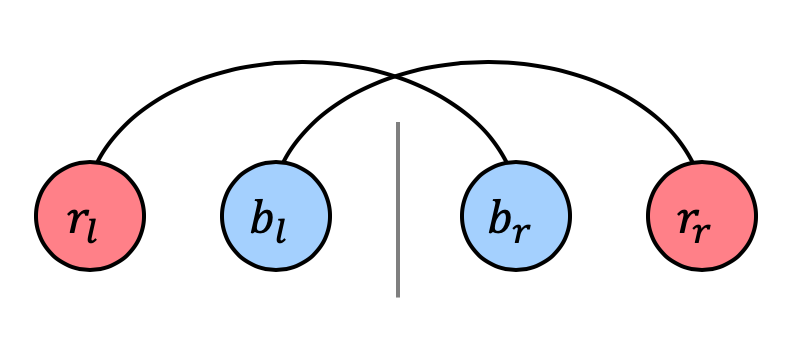
\includegraphics[height=2.5cm]{./images/colorblind3.png}\label{fig:f1}}
  \hfill
  \subfloat[จับคู่ฝั่งเดียวกัน cost = 2]{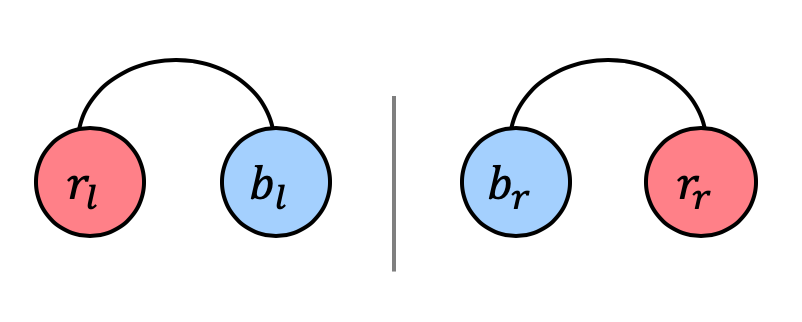
\includegraphics[height=2.3cm]{./images/colorblind2.png}\label{fig:f2}}
  \hfill
\end{figure}

ในรูปข้างล่าง เราพยายามที่จะจับคู่ในฝั่งซ้ายให้หมดก่อน ซึ่งจะเหลือจุดสีฟ้า 2 จุด ที่จะต้องไปจับคู่กับฝั่งขวา

\begin{figure}[h]
  \centering
  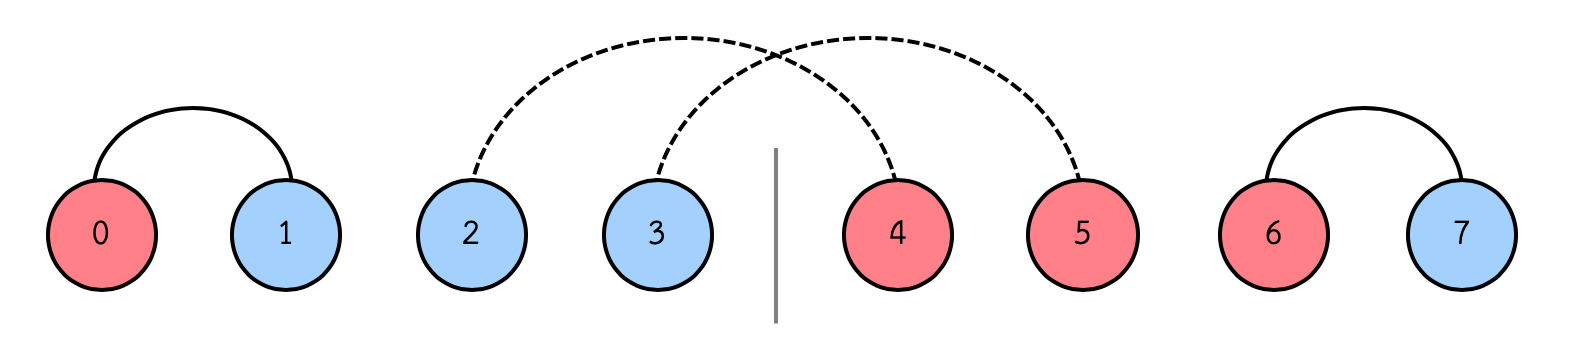
\includegraphics[height=3cm]{./images/colorblind1.png}
\end{figure}

\fbox{\parbox{12.85cm}{
Minimum total cost ในการจับคู่ของอาเรย์นี้ จะเท่ากับ $|R_0 - B_0| + ... + |R_{2N-2} - B_{2N-2}|$
}}

\newpage
\subsection{Subtask 3}

\underline{เงื่อนไขเพิ่มเติม}: ตำแหน่งที่มีสีฟ้าอยู่ติดกันหมด

เรารู้ว่าอาเรย์ของเราจะมีหน้าตาเป็นดังนี้ \code{"R..R\underline{B..B}R..R"} กำหนดให้ส่วนแรกที่เป็นสีแดงมีจำนวน $k$ ตัว

สังเกตุว่าค่า $R_i - B_i$ จะมีลักษณะเป็น $0, ..., k, k-1, ..., k-N, k-N+1, ..., 0$ 

\begin{figure}[h]
  \centering
  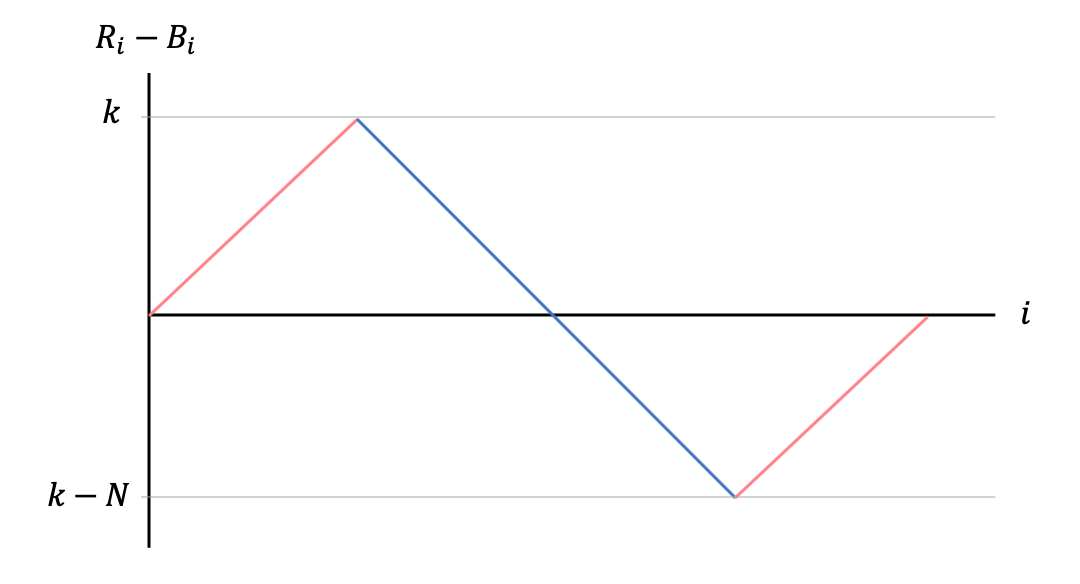
\includegraphics[height=4cm]{./images/colorblind4.png}
\end{figure}

สังเกตุว่าในจุดยอดของกราฟจะเป็นตำแหน่งที่จุดสีแดงและสีฟ้าอยู่ติดกันซึ่งเป็นตำแหน่งที่เราต้องหา หากเราลองสลับสีแดงและฟ้าที่ติดกันเราจะเห็นว่ามันจะทำให้ minimum total cost น้อยลงจาก minimum total cost ของอาเรย์ดั้งเดิมดังรูป

\begin{figure}[h]
  \centering
  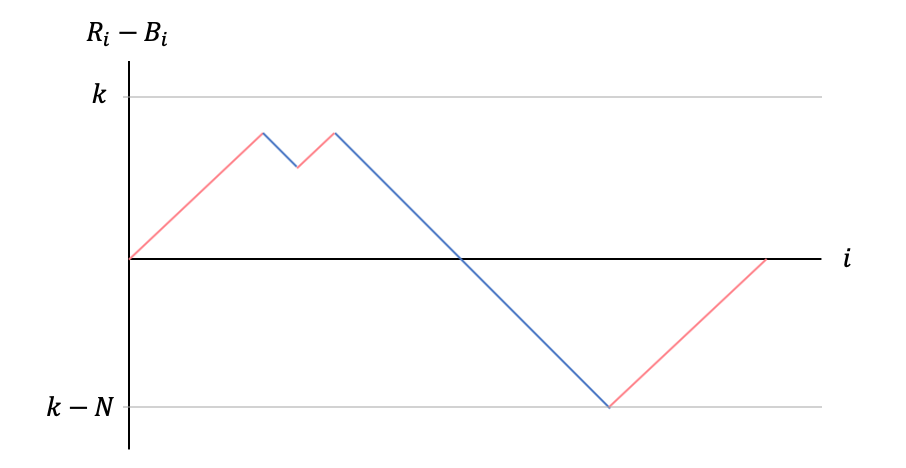
\includegraphics[height=4cm]{./images/colorblind5.png}
\end{figure}

อย่างไรก็ตาม หากอาเรย์คือ \code{"R\underline{B..B}R..R"} การสลับ \code{"R"} กับ \code{"B"} คู่แรกจะไม่ทำให้ minimum total cost ลดลง เราต้องเช็คกรณีนี้เป็นพิเศษ

ทีนี้ เราจะหา minimum total cost ของอาเรย์ดั้งเดิมได้ยังไง ค่านั้นจะเท่ากับ \code{ask(0,1)} เสมอ เพราะว่าอย่างที่ได้กล่าวไป การสลับคู่แรกของอาเรย์จะไม่เปลี่ยนค่า cost ของการจับคู่ใดๆ ถึงแม้ว่าสีที่สลับจะต่างกัน

เราต้องการหาตำแหน่งแรกที่สีต่างกันโดยการถาม \code{ask(i-1,i)} ไปเรื่อยๆตั้งแต่ \code{i} = $2, 3, ..., N$ \\\ หาก \code{ask(i-1,i)} ≠ \code{ask(0,1)} แสดงว่าที่ตำแหน่ง \code{i} เป็นตำแหน่งแรกของจุดสีฟ้า

Total query: $N$

\subsection{Subtask 4}

\underline{เงื่อนไขเพิ่มเติม}: ตำแหน่ง $2x$ และ $2x+1$ มีสีแตกต่างกัน สำหรับทุก $0 \leq x \leq N-1$

เนื่องจาก ตำแหน่ง $2x$ และ $2x+1$ ใดๆมีสีแตกต่างกัน เราสามารถสรุปได้ว่าตำแหน่งที่ 1 มีสีฟ้า %และ ค่า $R_i - B_i$ ของ $i$ ที่เป็นเลขคี่จะเท่ากับ 0 เสมอ

สังเกตุว่า หากเราถาม \code{ask(0,x)} โดยที่ \code{x} เป็นจำนวนคู่ แล้วจะเกิดได้สองกรณีดังนี้

\begin{enumerate}
  \item ตำแหน่ง \code{x} เป็นสีแดง: \code{ask(0,x)} จะเท่ากับ minimum total cost ของอาเรย์เดิม เนื่องจากเราสลับสีแดงกับสีแดง อาเรย์ยังคงเหมือนเดิม
  \item ตำแหน่ง \code{x} เป็นสีฟ้า: \code{ask(0,x)} จะมากกว่ากับ minimum total cost ของอาเรย์เดิมแน่นอน เนื่องจากอาเรย์จะเปลี่ยนจาก \code{"\underline{R}B..\underline{B}R.."} เป็น \code{"\underline{B}B..\underline{R}R.."} ซึ่งทำให้ต้องใช้ cost เพิ่มขึ้นในการจับคู่ 
\end{enumerate}

ดังนั้นในส่วนของการหาอาเรย์ เราสามารถสรุปได้ว่าสำหรับ \code{x} = $2, 4, ..., 2N-2$ หาก \code{ask(i-1,i)} = \code{ask(0,1)} แสดงว่าตำแหน่ง \code{x} และ \code{x+1} จะเป็น \code{"RB"} ไม่เช่นนั้นจะเป็น \code{"BR"}

Total query: $N$

\subsection{Subtask 5}

\underline{เงื่อนไขเพิ่มเติม}: ตั้งแต่ตำแหน่ง $0$ ถึง $N$ มีตำแหน่งสีฟ้าหนึ่งตำแหน่งพอดี

ในปัญหาย่อยนี้เราจะทำการสังเกตุค่าหากเราสลับตำแหน่ง $i$ กับ $N$ สังเกตุว่าหากอาเรย์เป็น \code{"R..RB..B"} แล้ว minimum total cost จะมีค่ามากที่สุด ดังนั้นหาก \code{ask(i,N) > ask(0,1)} แล้ว แสดงว่าที่ตำแหน่ง \code{i} เป็นสีฟ้า หากไม่มี \code{i} ใดๆที่ตรงเงื่อนไขแล้ว ตำแหน่ง $N$ จะเป็นสีฟ้า

Total query: $N$

\subsection{Subtask 6}

\underline{เงื่อนไข}: ไม่มีเงื่อนไขเพิ่มเติม

เราจะแบ่งอัลกอริธึมออกเป็นสองส่วน โดยในเฉลยนี้ขอแทนตำแหน่งสีแดงด้วย + และ สีฟ้าด้วย - ดังนั้น $R_i - B_i$ จะเท่ากับผลรวม $i$ ตำแหน่งแรก ขอแทนด้วย $pref_i$

\subsubsection{หาสีของ 3 ตำแหน่งแรก}

ใน 3 ตำแหน่งแรกนี้เป็นไปได้ 4 กรณีได้แก่ +++, ++-, +-+ และ +{-}{-} นอกจากนี้ สังเกตุว่าหากเราสลับตำแหน่งระหว่างสองตัวใดๆในสามตำแหน่งนี้ ค่า $pref_i$ สำหรับ $3 \leq i$ จะไม่เปลี่ยน ดังนั้นในตอนที่เราสลับคู่ใดๆ เราจะสนใจเพียงค่าที่เปลี่ยนไปของ $pref_1$ และ $pref_2$ ซึ่งเท่ากับค่า minimum total cost ที่เปลี่ยนไป

กำหนดให้ \code{C} เท่ากับ minimum total cost เริ่มต้น ซึ่งมีค่าเท่ากับ \code{ask(0,1)}

\newpage

\begin{table}[h]
\centering
\begin{tabular}{ | m{2cm} | P{2cm} | P{2cm} | P{2cm} |} 
\hline
& \code{ask(0,1) - C} & \code{ask(0,2) - C} & \code{ask(1,2) - C} \\ 
\hline
$+++$& 0 & 0 & 0 \\ 
\hline
$++-$& 0 & -2 & -2 \\ 
\hline
$+-+$& 0 & 0 & +2 \\ 
\hline
$+--$& 0 & +2 & 0 \\ 
\hline
\end{tabular}
\end{table}

ตารางดังกล่าวแสดงค่าที่เปลี่ยนไปของ minimum total cost (\code{ask(?,?) - C}) ซึ่งแสดงให้เห็นว่าเราสามารถที่จะแยกทั้ง 4 กรณีออกได้เพียงการถามแค่ 3 ครั้งเท่านั้น

\subsubsection{หาสีของตำแหน่งถัดๆไป}

สมมติว่าเรารู้สีของทุกตำแหน่งตั้งแต่ 0 ถึง $i-1$ แล้ว เราจะสามารถหาสีของตำแหน่ง $i$ โดยแบ่งกรณีจากสีของสองตำแหน่งล่าสุด (ตำแหน่ง $i-2$ และ $i-1$) และ ผลรวมของสีก่อนหน้านั้น ($pref_{i-3}$)

กำหนดให้ $\underline{?}$ เป็นสีของตำแหน่ง $i$ ที่เรากำลังจะหา

\begin{itemize}
  \item กรณี $++\underline{?}$ 

  \begin{table}[h]
  \centering
  \begin{tabular}{ | m{2cm} | P{1cm} | P{1cm} | P{1cm} | P{1cm} |} 
  \hline 
  \multirow{2}{4em}{\footnotesize{$pref_{i-3}$}} & \multicolumn{2}{c|}{\code{ask(i-1, i) - C}} & \multicolumn{2}{c|}{\code{ask(i-2, i) - C}} \\\cline{2-5}
  & $++\underline{+}$ & $++\underline{-}$ & $++\underline{+}$ & $++\underline{-}$\\
  \hline
  \footnotesize{$\geq 0$} & 0 & -2 & \cellcolor{gray!25} & \cellcolor{gray!25}\\ 
  \hline
  \footnotesize{$-1$} & \cellcolor{gray!25} & \cellcolor{gray!25} & 0 & -4 \\ 
  \hline
  \footnotesize{$\leq -2$} & \cellcolor{gray!25} & \cellcolor{gray!25} & 0 & +4 \\ 
  \hline
  \end{tabular}
  \end{table}

  \item กรณี $+-\underline{?}$ 

  \begin{table}[h]
  \centering
  \begin{tabular}{ | m{2cm} | P{1cm} | P{1cm} | P{1cm} | P{1cm} |} 
  \hline 
  \multirow{2}{4em}{\footnotesize{$pref_{i-3}$}} & \multicolumn{2}{c|}{\code{ask(i-1, i) - C}} & \multicolumn{2}{c|}{\code{ask(i-2, i) - C}} \\\cline{2-5}
  & $+-\underline{+}$ & $+-\underline{-}$ & $+-\underline{+}$ & $+-\underline{-}$\\
  \hline
  \footnotesize{$\geq 0$} & +2 & 0 & \cellcolor{gray!25} & \cellcolor{gray!25}\\ 
  \hline
  \footnotesize{$\leq -1$} & \cellcolor{gray!25} & \cellcolor{gray!25} & 0 & +4 \\ 
  \hline
  \end{tabular}
  \end{table}

\end{itemize}

ส่วนกรณีที่เป็น $-+\underline{?}$ และ $--\underline{?}$ สังเกตุว่าการสลับ $+$ และ $-$ ของทั้งอาเรย์ไม่ทำให้ minimum total cost เปลี่ยนไปเลย ดังนั้นเพียงกลับกรณี $++$ เป็น $--$ และ $+-$ เป็น $-+$ ได้เลย

ดังนั้น เราสามารถถามเพียง 1 คำถามเพื่อหาตัวถัดไปโดยแยกกรณีตามด้านบนได้

Total query: $3 + (2N - 3) = 2N$

\newpage





























\section{Coins}

สนามแห่งหนึ่งมีลักษณะเป็นวงกลม และ มีตำแหน่งเก็บเหรียญจำนวน $N$ ตำแหน่งโดยระยะห่างระหว่างตำแหน่ง $i$ และ $i+1$ เท่ากับ $A_i$ สำหรับ $1 \leq i < N$ และ ระยะห่างระหว่างตำแหน่ง $N$ และ $1$ เท่ากับ $A_N$ ที่ตำแหน่ง $i$ จะมีเหรียญหนึ่งเหรียญซึ่งมีเลข $B_i$ กำกับอยู่ซึ่งเลขซ้ำกันได้

\begin{figure}[h]
  \centering
  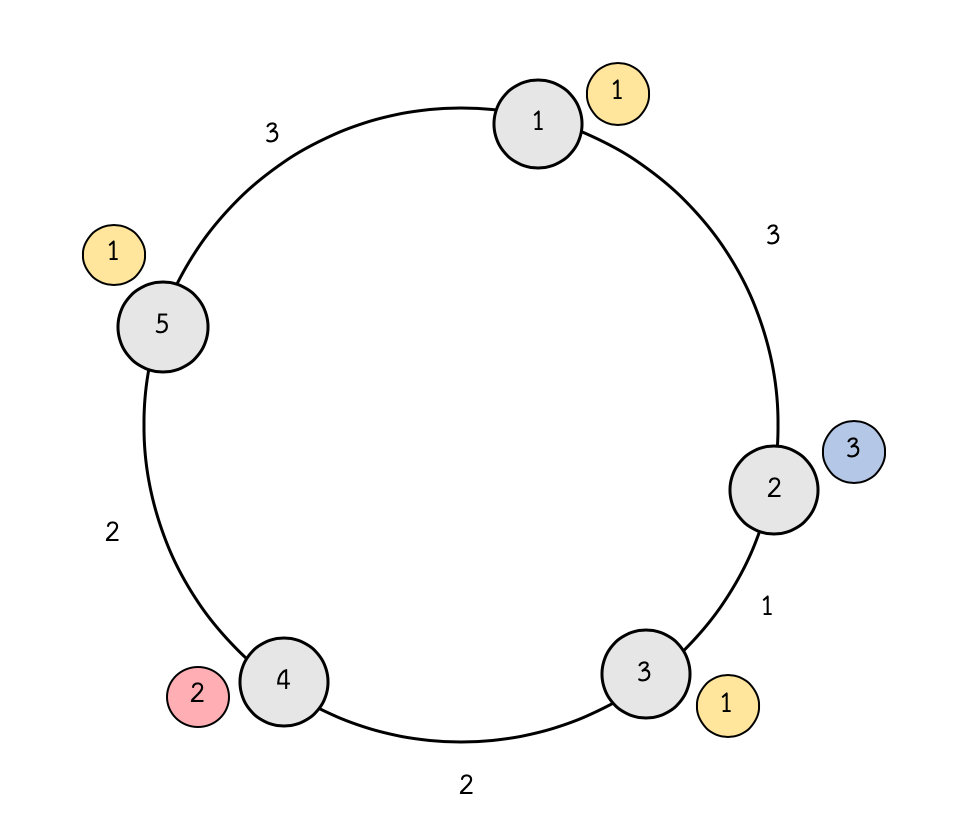
\includegraphics[height=4cm]{./images/coins1.png}  
  \captionsetup{labelformat=empty}
  \caption{ตัวอย่างสนามวงกลมที่มี 5 ตำแหน่ง}
\end{figure}

เราต้องการที่จะเก็บเหรียญตามลำดับจากเลขน้อยสุดไปยังมากสุด ถ้ามีเหรียญที่มีเลขซ้ำกันจะต้องเก็บเหรียญหมายเลขนั้นให้หมดก่อนถึงจะไปเก็บเหรียญที่มีเลขมากกว่าได้ จุดเริ่มต้นและจุดสิ้นสุดจะเริ่มที่ไหนก็ได้

ถามว่าระยะทางสั้นที่สุดที่เราจะใช้ในการเก็บเหรียญให้ครบเท่ากับเท่าใด

\underline{ข้อจำกัด}: $3 \leq N \leq 10^6$, $A_i \leq 10^8$ และ ผลรวม $A_i \leq 10^9$

\subsection{Subtask 1}

\underline{เงื่อนไขเพิ่มเติม}: $N \leq 10$

เราสามารถ Brute force ทดลองลำดับในการเดินไปเก็บเหรียญทุกลำดับได้ ​ซึ่งมีจำนวน $N!$ แบบ

Total time complexity: $\mathcal{O}(N!)$

\subsection{Subtask 2}

\underline{เงื่อนไขเพิ่มเติม}: เหรียญแต่ละหมายเลขมีจำนวนไม่เกิน 2 เหรียญ

เราจะใช้ dynamic programming (DP) ในการแก้ปัญหาโดยแบ่งเป็นสองจังหวะ

\begin{enumerate}[leftmargin=*]
  \item $st_x$ ระยะทางน้อยที่สุดโดยที่เหรียญที่เก็บล่าสุดอยู่ที่ ตำแหน่ง $x$ และเป็นตำแหน่ง\underline{แรก}ที่เก็บเหรียญหมายเลข $B_x$

  หากเราเก็บเหรียญหมายเลข $B_x - 1$ หมดแล้วและจบที่ตำแหน่ง $y$ เราจะเดินมายังเหรียญหมายเลข $B_x$
  $$
  st_x = \min
  \begin{cases}
    ft_y + walk(y, x) \\
    ft_y + walk(x, y)
  \end{cases}
  \text{โดย   } B_y = B_x - 1
  $$

  กำหนดให้ $walk(u,v)$ แทนระยะทางที่เดินจาก $u$ ไป $v$ ตามเข็มนาฬิกา
  \item $ft_x$ ระยะทางน้อยที่สุดโดยที่เหรียญที่เก็บล่าสุดอยู่ที่ ตำแหน่ง $x$ และเป็นตำแหน่ง\underline{สุดท้าย}ที่เก็บเหรียญหมายเลข $B_x$
  
  ส่วนนี้คือส่วนที่เราเริ่มเก็บเหรียญหมายเลข $B_x$ ตำแหน่งแรกที่ $y$ แล้ว เราต้องการเก็บเหรียญหมายเลขนี้ให้หมดแล้วมาหยุดที่ตำแหน่ง $x$ นี้
  $$
  ft_x = \min(st_y + collect(y,x)) \text{  โดย  } B_y = B_x
  $$

  โดย $collect(u,v)$ แทนระยะทางที่น้อยที่สุดที่ต้องใช้หากเราจะเก็บเหรียญหมายเลข $B_u$ ให้หมด โดยเริ่มเก็บที่ตำแหน่ง $u$ และจบที่ตำแหน่ง $v$ ($B_u = B_v$)
\end{enumerate}

ในปัญหาย่อยนี้ เนื่องจากเหรียญแต่ละหมายเลขมีจำนวนไม่เกิน 2 ดังนั้นในการคำนวณจึงมีตัวเลือกน้อย และ $collect(u,v)$ สามารถหาได้ง่ายมากเนื่องจากไม่ต้องไปเก็บเหรียญใดๆอื่นนอกจากจุดเริ่มและจบ (ตามเข็ม หรือ ทวนเข็มนาฬิกา)

คำตอบคือ $ft_i$ สำหรับ $i$ ที่ $B_i$ = เหรียญที่มีเลขมากที่สุด

\begin{lstlisting}[language=C++]
long long walk(int x, int y) {
  if(y >= x) return pos[y] - pos[x];
  return circ + pos[y] - pos[x];
}

long long solve() {
  for(int x = 1; x <= n; x++) {
    m = max(m, B[x]);
    coins[B[x]].push_back(x);
    st[x] = ft[x] = inf;
  }
  for(int i = 1; i <= m; i++) {
    // solve for st[x]
    for(auto x : coins[i]) {
      for(auto y : coins[i-1]) st[x] = min(st[x], ft[y] + min(walk(y, x), walk(x, y)));
      if(i == 1) st[x] = 0;
    }
    // solve for ft[x]
    int sz = coins[i].size();
    if(sz == 1) ft[coins[i][0]] = st[coins[i][0]];
    else {
      for(auto x : coins[i]) {
        for(auto y : coins[i]) {
          if(x != y) ft[x] = min(ft[x], st[y] + min(walk(y, x), walk(x, y)));
        }
      }
    }
  }
  long long ans = inf;
  for(auto x : coins[m]) ans = min(ans, ft[x]); 
  return ans;
}
\end{lstlisting}

Total time complexity: $\mathcal{O}(N)$

\subsection{Subtask 3}

\underline{เงื่อนไขเพิ่มเติม}: $N \leq 10\,000$, เหรียญแต่ละหมายเลขมีจำนวนไม่เกิน $1\,000$ เหรียญ และ ระยะห่างระหว่างเหรียญที่ติดกันเป็น 1 หมด

เราจะแก้ปัญหาด้วย DP เช่นเดียวกัน แต่ในปัญหาย่อยนี้ การหาค่า $collect(y, x)$ นั้นจะยากขึ้น

การเก็บเหรียญบนวงกลมที่ดีที่สุดนั้นทำได้อย่างไร ?

\begin{figure}[h]
  \centering
  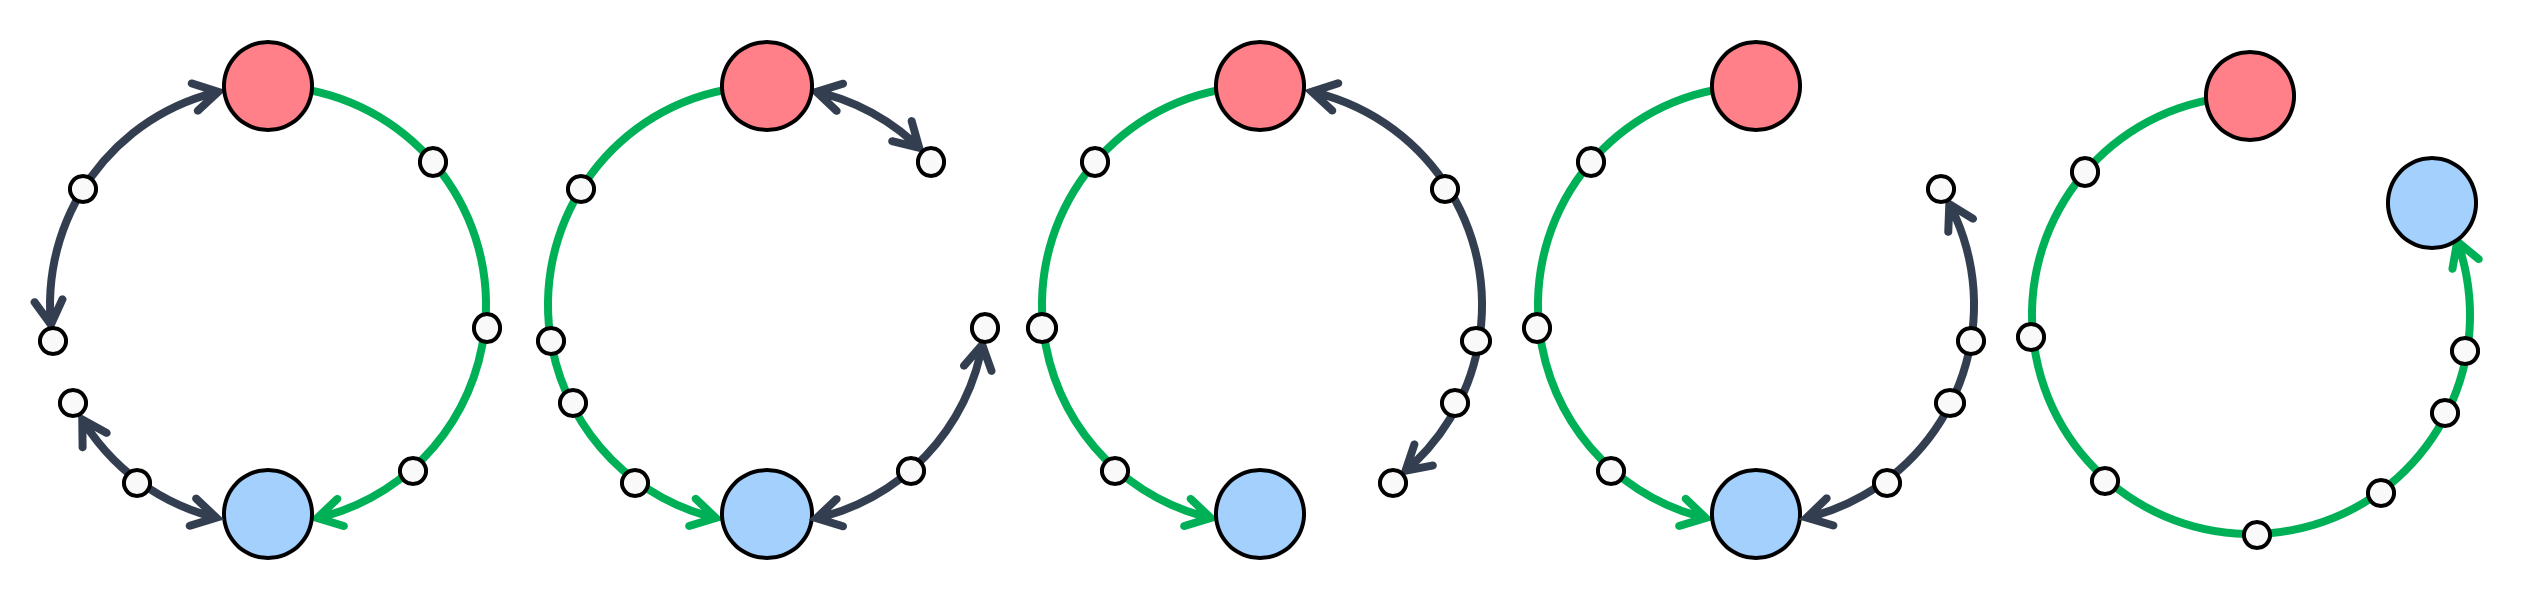
\includegraphics[height=3.3cm]{./images/coins2.png}
\end{figure}

รูปข้างต้นเป็นตัวอย่างวิธีเดินเก็บเหรียญที่เป็นไปได้ หากเราต้องการเก็บเหรียญทั้งหมดโดยเริ่มจากสีแดงและจบที่สีฟ้า

การเดินเก็บเหรียญตามด้านบนจะมีลักษณะดังนี้
\begin{itemize}
  \item \textbf{สีดำ}: เดินไปเก็บเหรียญจำนวนหนึ่งแล้วเดินกลับ (อาจไม่มี)
  \item \textbf{สีเขียว}: เดินไปเก็บไปถึงตำแหน่งสีฟ้า
  \item \textbf{สีดำ}: เดินเลยจากสีฟ้าไปเก็บเหรียญที่ยังเหลืออยู่แล้วเดินกลับ (อาจไม่มี)
\end{itemize}

\fbox{\parbox{12.85cm}{
ในการคำนวณในส่วน 2 เราจะสนใจเพียงกรณีที่ \underline{จุดเริ่มและจุดจบอยู่ติดกันในวงกลม}
เนื่องจาก 
\\\ เราไม่จำเป็นจะต้องสนใจส่วนสีดำเนื่องจากส่วนนั้นเราสามารถให้ส่วน 1 นั้นเลือกแทนได้
}}

\begin{figure}[h]
  \centering
  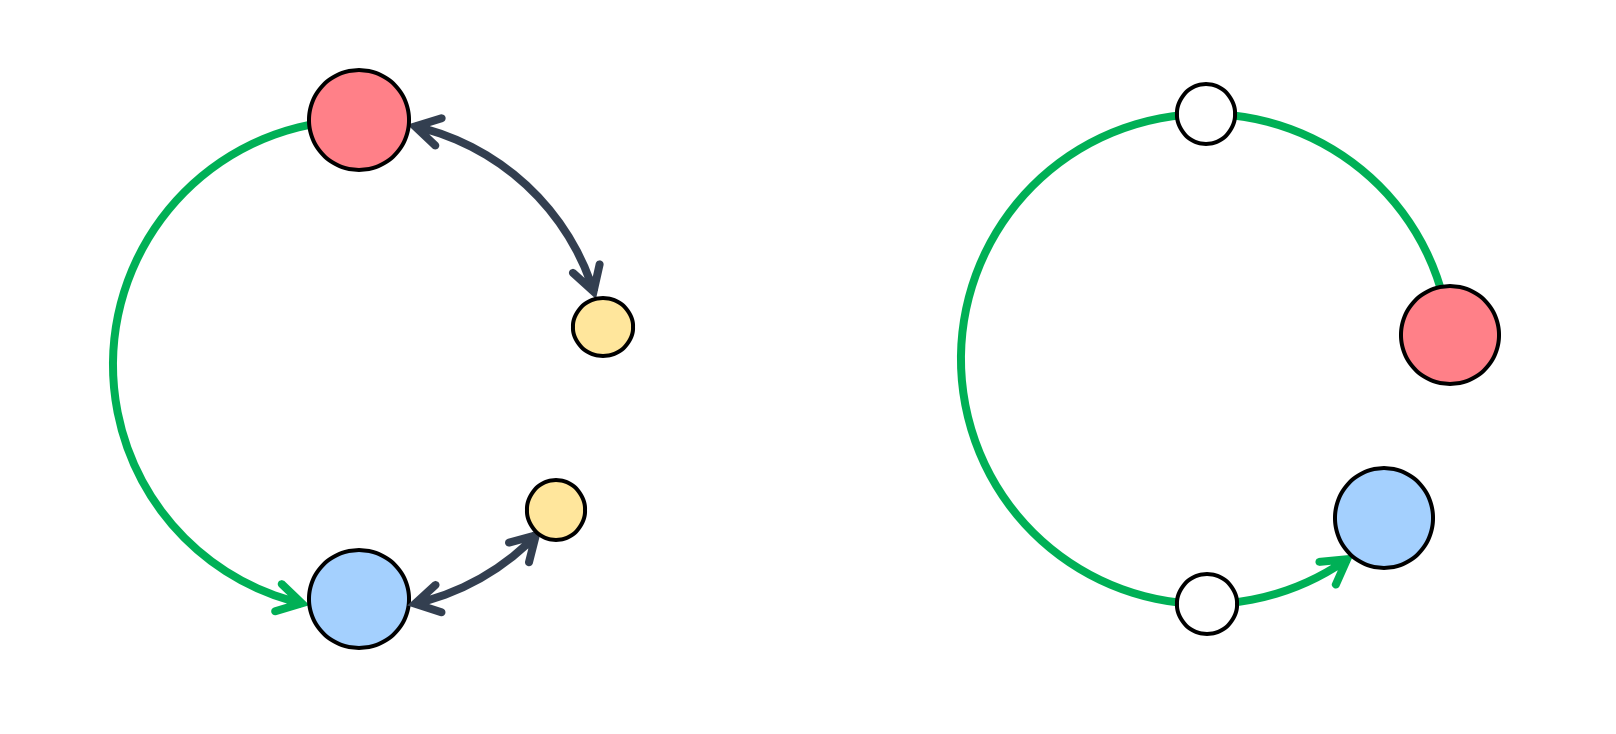
\includegraphics[height=3.5cm]{./images/coins3.png}
\end{figure}

ตัวอย่างเช่น จากรูปข้างบน แทนที่จะเดินไปกลับ หากเราย้ายจุดเริ่มและจุดจบมาที่จุดสีเหลืองแทน แล้วปล่อยให้การตัดสินใจเดินผ่านทางสีดำนั้นเป็นหน้าที่ของส่วนที่ 1 ซึ่งคือการเดินมาจากเหรียญหมายเลขต่ำกว่า

\newpage
ดังนั้นการหาระยะทางจะมีเพียงสองแบบ

\begin{figure}[h]
  \centering
  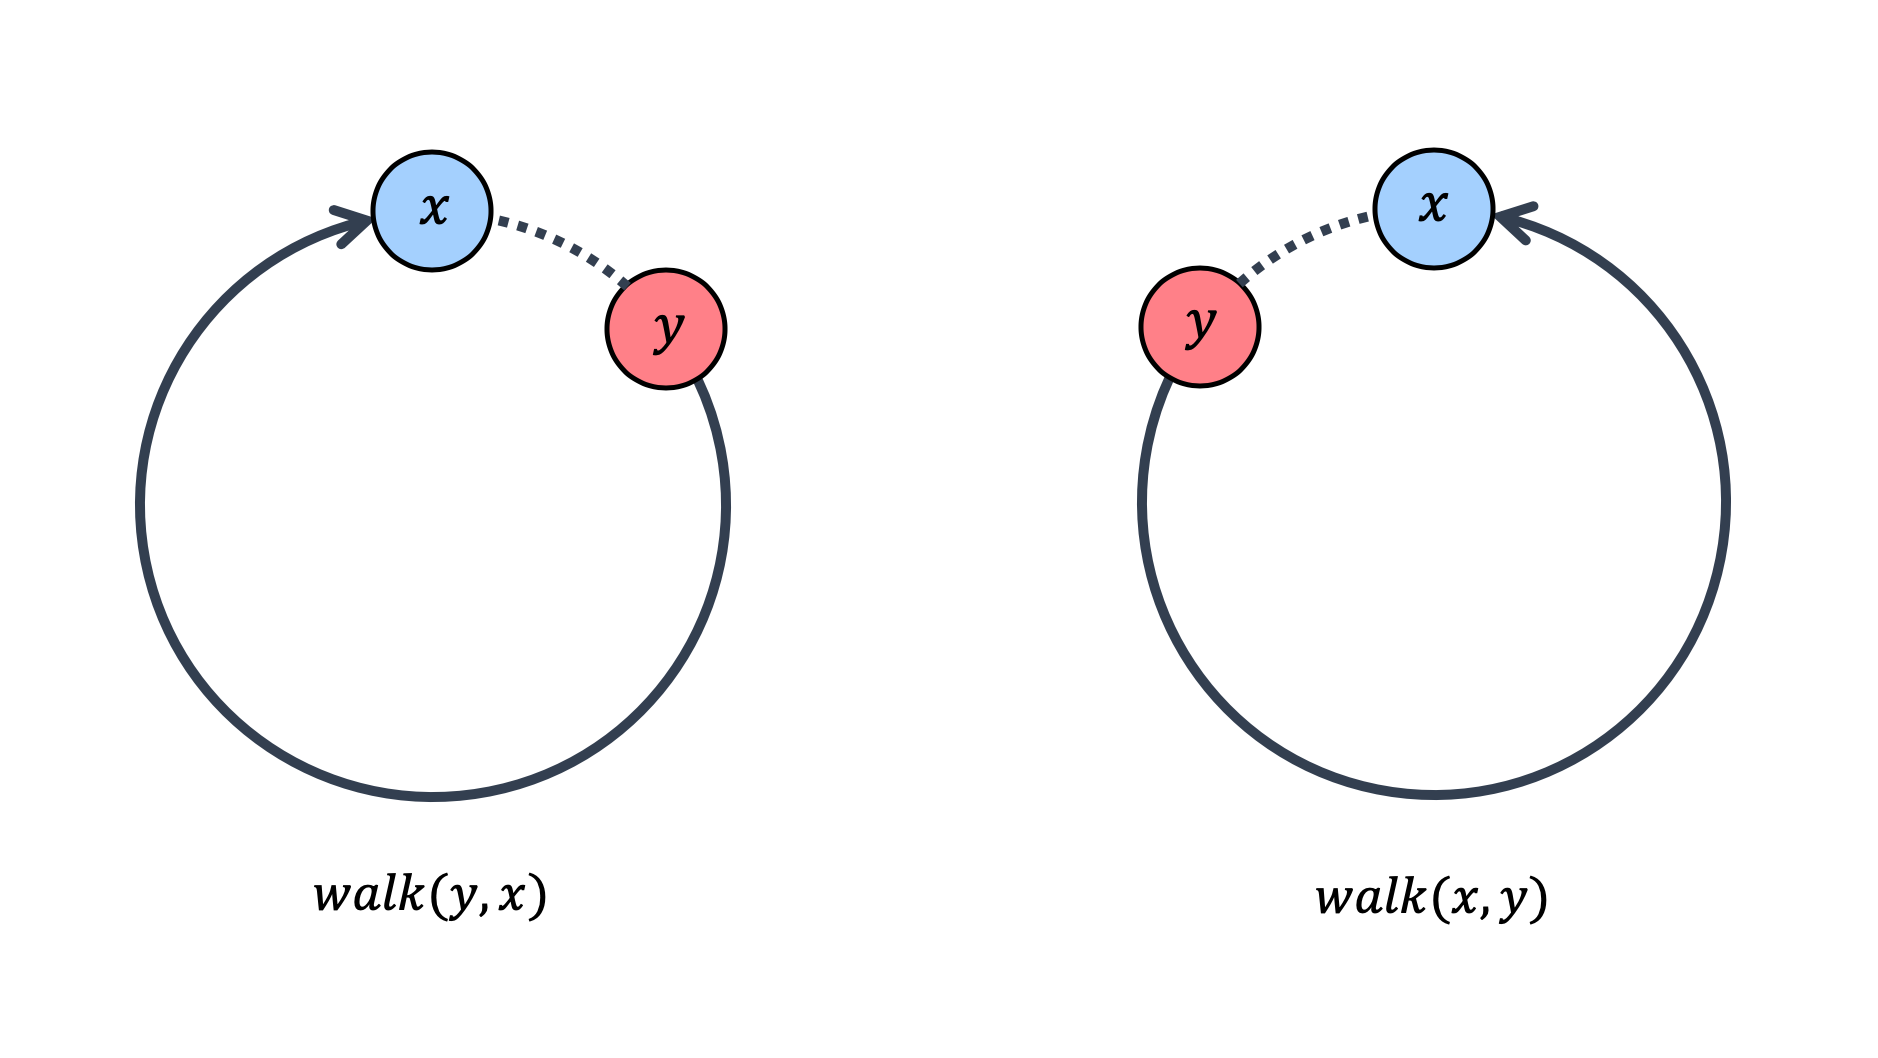
\includegraphics[height=4.5cm]{./images/coins4.png}
\end{figure}

หาก $x$ อยู่ก่อน $y$ ในวงกลมแล้วเราจะต้องใช้ระยะทาง $walk(y, x)$ ไม่เช่นนั้นเราจะเดินย้อนอีกทางซึ่งเป็น $walk(x, y)$ ทั้งนี้ทิศทางการเดินนั้นขึ้นอยู่กับด้านที่ต้องไปเก็บเหรียญอื่นๆ

\begin{lstlisting}[language=C++]
// solve for ft[x]
int sz = coins[i].size();
if(sz == 1) ft[coins[i][0]] = st[coins[i][0]];
else {
  for(int j = 0; j < sz; j++) {
    int x = coins[i][j], y;

    y = coins[i][(j+1)%sz];
    ft[x] = min(ft[x], st[y] + walk(y, x)); // walk from y to x clockwise

    y = coins[i][(j-1+sz)%sz];
    ft[x] = min(ft[x], st[y] + walk(x, y)); // walk from y to x counter-clockwise
  }
}
\end{lstlisting}

Total time complexity: $\mathcal{O}(N^2)$

\newpage

\subsection{Subtask 4 และ 5}

\underline{เงื่อนไข}: ไม่มีเงื่อนไขเพิ่มเติม

พิจารณา $st_x = \min(ft_y + \min(walk(y,x), walk(x,y)))$ ซึ่งแบ่งเป็นสองกรณี

\begin{enumerate}[leftmargin=*]
  \item $x \geq y$

  $
  st_x = \min
  \begin{cases}
    ft_y + walk(y, x) = {\setlength{\fboxsep}{2pt}\fbox{$\displaystyle ft_y - pos_y$}} + pos_x \\
    ft_y + walk(x, y) = {\setlength{\fboxsep}{2pt}\fbox{$\displaystyle ft_y + C + pos_y$}} - pos_x
  \end{cases}
  $

  \item $x < y$

  $
  st_x = \min
  \begin{cases}
    ft_y + walk(y, x) = {\setlength{\fboxsep}{2pt}\fbox{$\displaystyle ft_y + pos_y$}} - pos_x \\
    ft_y + walk(x, y) = {\setlength{\fboxsep}{2pt}\fbox{$\displaystyle ft_y + C - pos_y$}} + pos_x
  \end{cases}
  $
\end{enumerate}

โดย $C$ แทน เส้นรอบวงของสนาม $= \sum A$

เนื่องจากเราต้องการให้ $st_x$ มีค่าน้อยที่สุดดังนั้น เราจะหา $ft_y + pos_y$ หรือ $ft_y + C - pos_y$ ที่น้อยที่สุดหาก $x \leq y$ และ หา $ft_y - pos_y$ หรือ $ft_y + C + pos_y$ ที่น้อยที่สุดหาก $x > y$

ซึ่งเราสามารถใช้เทคนิค two pointer ในการหาค่าน้อยที่สุดได้ โดยเราจะค่อยๆไล่ค่า $x$ จากน้อยไปมาก และ ค่อยๆเพิ่ม $y$ ที่ $\leq x$ และจำค่าที่น้อยที่สุดของ $ft_y - pos_y$ และ $ft_y + C + pos_y$ ที่น้อยที่สุด เพื่อมาคำนวณ \\\
และทำเช่นเดียวกันกับกรณี $x<y$ โดยการไล่ค่า $x$ จากมากไปน้อย

\begin{lstlisting}[language=C++]
// case x >= y
int l = -1; // this is a pointer for y so that coins[i-1][l] <= x
long long mn1 = inf, mn2 = inf;

// iterate x in increasing order
for(auto x : coins[i]) {
  // gradually increase pointer for y
  while(l+1 < coins[i-1].size() && coins[i-1][l+1] <= x) {
    l++; int y = coins[i-1][l]; 
    mn1 = min(mn1, ft[y] - pos[y]); 
    mn2 = min(mn2, ft[y] + circ + pos[y]);
  }
  st[x] = min(st[x], mn1 + pos[x]); // ft[y] + walk(y, x) = ft[y] - pos[y] + pos[x]
  st[x] = min(st[x], mn2 - pos[x]); // ft[y] + walk(x, y) = ft[y] + circ + pos[y] - pos[x]
}

// case x < y
// do the similar thing as above
\end{lstlisting}

Total time complexity: $\mathcal{O}(N)$

\newpage



























\section{Castle}




มีกราฟขนาด $N$ โหนด ($0$ ถึง $N-1$) และ $M$ เส้นเชื่อม ($N-1 \leq M \leq N+9$) กราฟนี้จะมีลักษณะเป็นต้นไม้ไบนารี่สมบูรณ์ (full binary tree) ที่มีเส้นเชื่อมพิเศษเพิ่มมาอีก $M-N+1$ เส้น 

เราต้องเขียนโปรแกรมที่จะรองรับเหตุการณ์สองแบบ จำนวน $Q$ เหตุการณ์
\begin{enumerate}
  \item เส้นเชื่อมหนึ่งเส้นพังทลายลงไป
  \item ถามว่า $u$ และ $v$ มีทางเดินที่เชื่อมกันอยู่รึไม่
\end{enumerate}

โปรแกรมจะทำงานแบบ online ซึ่งหมายความว่าสำหรับเหตุการณ์คำถามเราต้องตอบคำถามก่อน​ถึงจะได้รับเหตุการณ์ต่อไป

\underline{ข้อจำกัด}: $1 \leq N, Q \leq 100\,000$ และ $N-1 \leq M \leq N+9$

\subsection{Subtask 1}

\underline{เงื่อนไขเพิ่มเติม}: $N \leq 1\,000, Q \leq 1\,000$

$u$ และ $v$ จะมีืทางเดินเชื่อมกันอยู่ หาก $u$ และ $v$ อยู่ใน component เดียวกัน ซึ่งเราสามารถใช้ DFS/BFS หรือว่า \href{https://en.wikipedia.org/wiki/Disjoint-set_data_structure}{Union-find disjoint set} เพื่อหาว่าแต่ละโหนดอยู่ใน component ใดบ้างได้ใน $\mathcal{O}(M)$

ดังนั้นในการตอบคำถามแต่ละครั้ง เราก็รันอัลกอริธึมบนกราฟเพื่อหาว่า $u$ และ $v$ อยู่ใน component \\\ เดียวกันรึเปล่า

Total time complexity: $\mathcal{O}(M*Q)$

\subsection{Subtask 2}

\underline{เงื่อนไขเพิ่มเติม}: $M = N-1$,  ต้นไม้ไบนารี่ของกราฟจะมีลักษณะเป็นเส้นเชื่อมโหนด $i$ กับ $\floor{\frac{i-1}{2}}$ สำหรับทุก $i > 0$

เราจะทำการระบายสีต้นไม้โดยที่ หากโหนดใดๆมีทางเดินไปหากันได้จะมีสีเดียวกัน แน่นอนว่าเริ่มแรกทุกโหนดจะมีสีเดียวกัน

หากเรานำเส้นเชื่อมในต้นไม้ใดๆออก มันจะทำการแบ่งกลุ่มของต้นไม้ออกเป็นสองกลุ่มย่อย ซึ่งสองกลุ่มนั้นจะไม่สามารถเดินทางไปหากันได้ ทำให้เราต้องระบายสีต้นไม้ใหม่

\begin{figure}[h]
  \centering
  \hfill
  \subfloat[เริ่มแรกต้นไม้มีสีเดียวกันหมด]{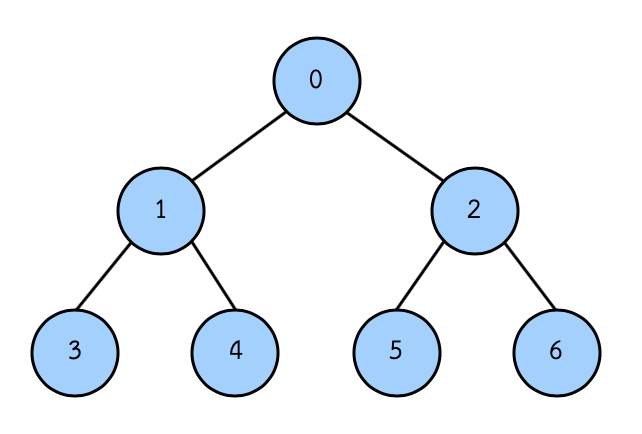
\includegraphics[height=3cm]{./images/castle1.png}}
  \subfloat[สีหลังจากตัดเส้นเชื่อม (0,1)]{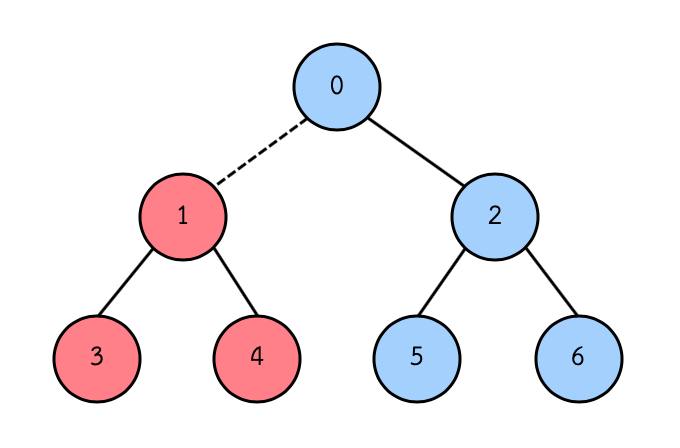
\includegraphics[height=3cm]{./images/castle2.png}}
  \subfloat[สีหลังจากตัดเส้นเชื่อม (2,5)]{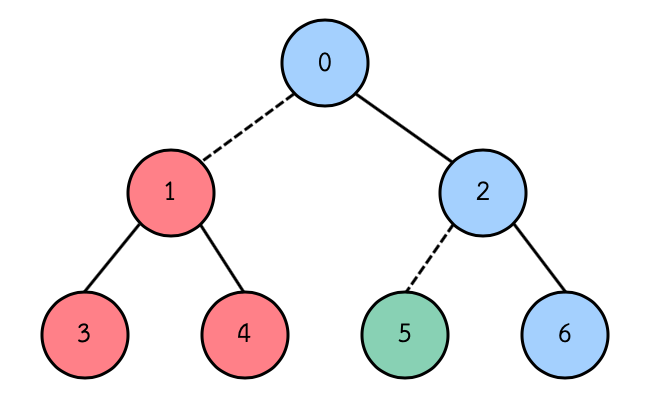
\includegraphics[height=3cm]{./images/castle3.png}}
  \hfill
\end{figure}

ทุกครั้งที่แบ่งจะแบ่งออกเป็นสองส่วนเสมอ ทีนี้เราต้องเลือกว่าจะระบายสีในส่วนไหนให้ดีที่สุด

\fbox{\parbox{12.85cm}{
หากเราระบายสีในส่วนที่อยู่ด้านล่างเสมอ เราจะทำการระบายสีโหนดใดๆไม่เกิน $\log N$ ครั้ง เนื่องจากต้นไม้เป็น full binary tree
}}

ในการระบายสี เราสามารถใช้ DFS/BFS ลงไปจากโหนดเริ่มต้นได้ตามตัวอย่างโค้ด C++ นี้

\begin{lstlisting}[language=C++]
// color the subtree rooted at u
void coloring(int u) {
  for(auto v : children[u]) {
    if(color[u] == color[v]) coloring(v);
  }
  color[u] = new_color;
}

// destroy an sedge between u and v
void cut(int u, int v) {
  new_color += 1; // initially, new_color = 0
  if(depth[u] > depth[v]) coloring(u);
  else coloring(v);
}
\end{lstlisting}

เท่านี้ในตอนตอบคำถาม เราเพียงแค่ดูว่า \code{color[u]} เท่ากับ \code{color[v]} รึเปล่าเท่านั้น

Total time complexity: $\mathcal{O}(N \log N + Q)$

\subsection{Subtask 3}

\underline{เงื่อนไขเพิ่มเติม}: $M = N-1$

ในปัญหาย่อยที่แล้วเรารู้ว่า root ของต้นไม้เป็น 0 เสมอ แต่ในปัญหาย่อยนี้เราจะต้องหาเอง

สังเกตุว่า root ของต้นไม้เป็นโหนดเดียวที่มีเส้นเชื่อมกับมันเท่ากับ 2 พอดี ดังนั้นเราสามารถหาได้เลยว่า root ของต้นไม้เป็นอะไรเพียงดูแค่ degree ของแต่ละ node

Total time complexity: $\mathcal{O}(N \log N + Q)$

\subsection{Subtask 4}

\underline{เงื่อนไขเพิ่มเติม}: $M = N$ และ ต้นไม้ไบนารี่ของกราฟจะมีลักษณะเป็นเส้นเชื่อมโหนด $i$ กับ $\floor{\frac{i-1}{2}}$ สำหรับทุก $i > 0$

ในปัญหาย่อยนี้มีลักษณะเหมือนกับปัญหาย่อยที่ 2 แต่มี เส้นเชื่อมพิเศษเพิ่มขึ้นมาอีก 1 เส้น กำหนดให้เส้นเชื่อมนี้เชื่อมระหว่างโหนด $a$ และ $b$

เราจะทำแบบเดียวกับที่ทำใน Subtask 2 นั่นคือสนใจก่อนว่าสีที่ถูกระบายในต้นไม้ของ $u$ และ $v$ นั้นเป็นสีเดียวกันหรือไม่ 

แต่ว่าเนื่องจากเรามีเส้นเชื่อมพิเศษระหว่างโหนด $a$ และ $b$ ดังนั้นกลุ่มโหนดที่มีสี \code{color[a]} จะสามารถเดินทางไปหากลุ่มสี \code{color[b]} ได้ ตรงนี้เราสามารถเช็คได้ตอนถามคำถามได้เช่นเลย

\begin{figure}[h]
  \centering
  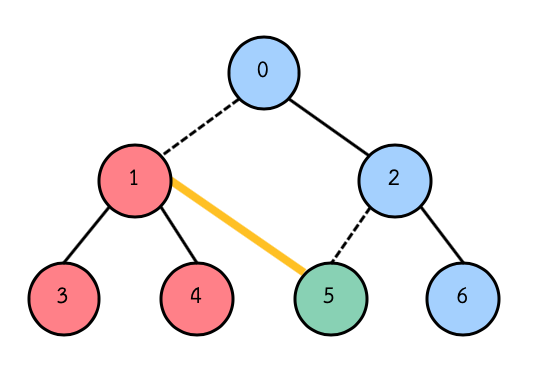
\includegraphics[height=3cm]{./images/castle4.png}
  \captionsetup{labelformat=empty}
  \caption{มีเส้นเชื่อมพิเศษระหว่าง 1 และ 5 ทำให้สีแดงและเขียวสามารถเดินทางหากันได้}
\end{figure}

\begin{lstlisting}[language=C++]
// query connectivity
bool query(int u, int v) {
  // same color in the tree
  if(color[u] == color[v]) return true;

  // special edge connects color[a] and color[b]
  if(special) { // check whether the special edge has been cut
    if(color[u] == color[a] && color[v] == color[b]) return true;
    if(color[u] == color[b] && color[v] == color[a]) return true;
  }
  
  return false;
}

// destroy an sedge between u and v
void cut(int u, int v) {
  // cut special edge
  if((u == a && v == b) || (u == b && v == a)) special = false
  // cut tree edge
  else {
    new_color += 1; // initially, new_color = n
    if(depth[u] > depth[v]) coloring(u);
    else coloring(v);
  }
}
\end{lstlisting}

Total time complexity: $\mathcal{O}(N \log N + Q)$

\subsection{Subtask 5}

\underline{เงื่อนไขเพิ่มเติม}: $M = N$

เช่นเดียวกันกับ Subtask 3 เราจะไม่รู้ว่าต้นไม้ไบนารี่นั้นมีลักษณะเป็นอย่างไร อย่างไรก็ตาม หากเราสังเกตุคุณสมบัติของ full binary tree ความสูง $k$ ที่มี $2^k-1$ โหนด ต้นไม้จะมีโหนด degree = 2 เพียง 1 โหนด degree = 1 จำนวน $2^{k-1}$ และ ที่เหลือมี degree = 3 

ดังนั้นถ้าสมมติเราทดลองเอาเส้นเชื่อมหนึ่งเส้นออกจากกราฟ แล้วโหนดทั้งหมดมีคุณสมบัติตามข้างต้น แสดงว่าเส้นเชื่อมนั้นเป็นเส้นเชื่อมพิเศษ

หลังจากรู้เส้นเชื่อมพิเศษแล้วก็ใช้วิธีเดียวกับ Subtask 3 และ 4 รวมกันในการแก้

Total time complexity: $\mathcal{O}(N \log N + Q)$

\subsection{Subtask 6}

\underline{เงื่อนไขเพิ่มเติม}: ต้นไม้ไบนารี่ของกราฟจะมีลักษณะเป็นเส้นเชื่อมโหนด $i$ กับ $\floor{\frac{i-1}{2}}$ สำหรับทุก $i > 0$

เนื่องจากในกราฟจะมีเส้นเชื่อมพิเศษไม่เกิน 10 เส้น ดังนั้นเราจะมีกลุ่มสีในต้นไม้ที่สนใจไม่เกิน 20 กลุ่ม 

หากเราเอา 20 กลุ่มนี้มาสร้างกราฟขนาด 20 โหนด เราจะรู้ว่ากลุ่มใดสามารถเดินไปหากลุ่มใดในกราฟขนาดเล็กนี้ได้

\begin{figure}[h]
  \centering
  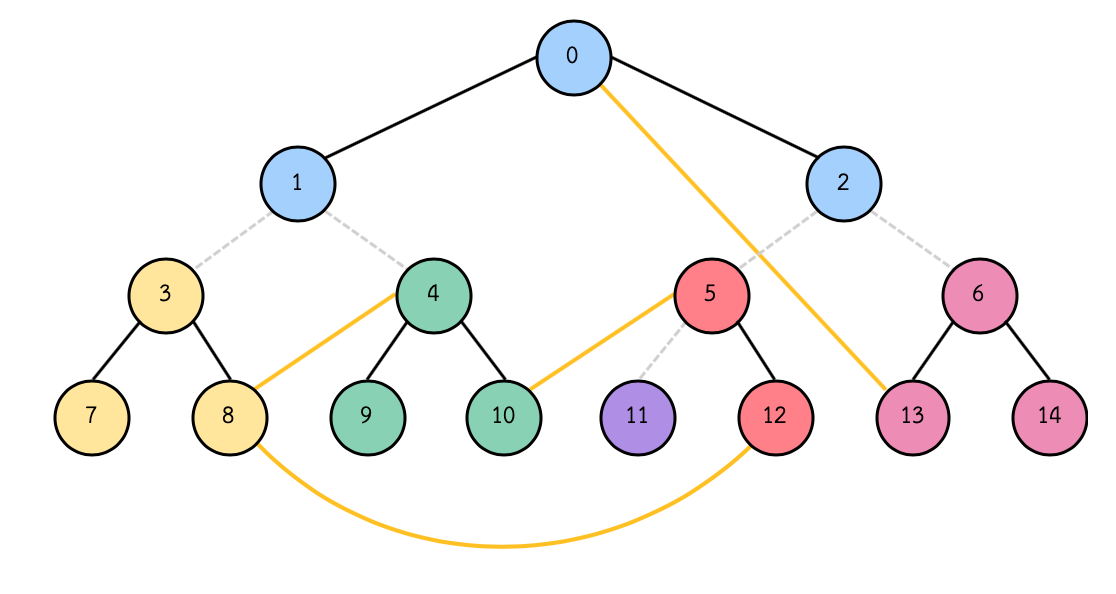
\includegraphics[height=5cm]{./images/castle5.png}
  \captionsetup{labelformat=empty}
  \caption{ต้นไม้และเส้นเชื่อมพิเศษสี่เส้น}
\end{figure}

\begin{figure}[h]
  \centering
  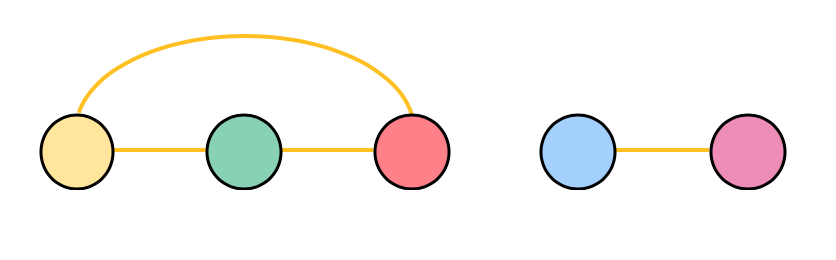
\includegraphics[height=2.5cm]{./images/castle6.png}
  \captionsetup{labelformat=empty}
  \caption{กราฟขนาดเล็กที่สร้างจากกลุ่มสีในต้นไม้และเส้นเชื่อมพิเศษข้างต้น}
\end{figure}

เช่น หากเราต้องการดูว่า 3 และ 5 สามารถเดินทางไปหากันได้รึเปล่า เราก็จะเช็คว่าสีของ 3 และ 5 ในต้นไม้ ซึ่งคือ สีเหลือง และ สีแดง สามารถเดินทางไปหากันได้รึเปล่าในกราฟขนาดเล็ก ซึ่งการเช็คนั้นเราก็สามารถที่จะใช้ DFS/BFS หรือว่า Disjoint set ได้เช่นเดิม

Total time complexity: $\mathcal{O}(N \log N + 20 * Q)$

\subsection{Subtask 7}

\underline{เงื่อนไข}: ไม่มีเงื่อนไขเพิ่มเติม

เนื่องจากเส้นเชื่อมพิเศษมีจำนวนไม่มาก (≤ 10 เส้น) หากเราเลือก spanning tree ใดๆ ออกมาจากกราฟ ต้นไม้นั้นจะยังมีลักษณะไม่ต่างจากต้นไม้ไบนารี่สมบูรณ์มาก ทำให้คุณสมบัติระบายสีไม่เกิน $\log N$ ครั้งต่อแต่ละโหนดที่ได้กล่าวไว้ใน Subtask 2 จึงยังมีผลอยู่

ดังนั้นในปัญหาย่อยนี้ เราเพียงเลือกต้นไม้ใดๆก็ได้ออกมาจากกราฟ แล้วทำลักษณะเช่นเดียวกับ Subtask 6 ได้เลย

Total time complexity: $\mathcal{O}(N \log N + 20 * Q)$

\subsection{Challenge}

ลองแก้ปัญหานี้หากกราฟมีลักษณะ\underline{แบบไหนก็ได้}ไม่จำเป็นต้องเป็นต้นไม้ไบนารี่สมบูรณ์ที่มีเส้นเชื่อมพิเศษเพิ่ม

ปัญหานี้สามารถแก้ได้ด้วยเวลา $\mathcal{O}(N \log N + 20 * Q)$ เช่นเดียวกัน

\end{document}
